\documentclass[twoside]{book}

% Packages required by doxygen
\usepackage{fixltx2e}
\usepackage{calc}
\usepackage{doxygen}
\usepackage[export]{adjustbox} % also loads graphicx
\usepackage{graphicx}
\usepackage[utf8]{inputenc}
\usepackage{makeidx}
\usepackage{multicol}
\usepackage{multirow}
\PassOptionsToPackage{warn}{textcomp}
\usepackage{textcomp}
\usepackage[nointegrals]{wasysym}
\usepackage[table]{xcolor}

% Font selection
\usepackage[T1]{fontenc}
\usepackage[scaled=.90]{helvet}
\usepackage{courier}
\usepackage{amssymb}
\usepackage{sectsty}
\renewcommand{\familydefault}{\sfdefault}
\allsectionsfont{%
  \fontseries{bc}\selectfont%
  \color{darkgray}%
}
\renewcommand{\DoxyLabelFont}{%
  \fontseries{bc}\selectfont%
  \color{darkgray}%
}
\newcommand{\+}{\discretionary{\mbox{\scriptsize$\hookleftarrow$}}{}{}}

% Page & text layout
\usepackage{geometry}
\geometry{%
  a4paper,%
  top=2.5cm,%
  bottom=2.5cm,%
  left=2.5cm,%
  right=2.5cm%
}
\tolerance=750
\hfuzz=15pt
\hbadness=750
\setlength{\emergencystretch}{15pt}
\setlength{\parindent}{0cm}
\setlength{\parskip}{3ex plus 2ex minus 2ex}
\makeatletter
\renewcommand{\paragraph}{%
  \@startsection{paragraph}{4}{0ex}{-1.0ex}{1.0ex}{%
    \normalfont\normalsize\bfseries\SS@parafont%
  }%
}
\renewcommand{\subparagraph}{%
  \@startsection{subparagraph}{5}{0ex}{-1.0ex}{1.0ex}{%
    \normalfont\normalsize\bfseries\SS@subparafont%
  }%
}
\makeatother

% Headers & footers
\usepackage{fancyhdr}
\pagestyle{fancyplain}
\fancyhead[LE]{\fancyplain{}{\bfseries\thepage}}
\fancyhead[CE]{\fancyplain{}{}}
\fancyhead[RE]{\fancyplain{}{\bfseries\leftmark}}
\fancyhead[LO]{\fancyplain{}{\bfseries\rightmark}}
\fancyhead[CO]{\fancyplain{}{}}
\fancyhead[RO]{\fancyplain{}{\bfseries\thepage}}
\fancyfoot[LE]{\fancyplain{}{}}
\fancyfoot[CE]{\fancyplain{}{}}
\fancyfoot[RE]{\fancyplain{}{\bfseries\scriptsize Generated by Doxygen }}
\fancyfoot[LO]{\fancyplain{}{\bfseries\scriptsize Generated by Doxygen }}
\fancyfoot[CO]{\fancyplain{}{}}
\fancyfoot[RO]{\fancyplain{}{}}
\renewcommand{\footrulewidth}{0.4pt}
\renewcommand{\chaptermark}[1]{%
  \markboth{#1}{}%
}
\renewcommand{\sectionmark}[1]{%
  \markright{\thesection\ #1}%
}

% Indices & bibliography
\usepackage{natbib}
\usepackage[titles]{tocloft}
\setcounter{tocdepth}{3}
\setcounter{secnumdepth}{5}
\makeindex

% Hyperlinks (required, but should be loaded last)
\usepackage{ifpdf}
\ifpdf
  \usepackage[pdftex,pagebackref=true]{hyperref}
\else
  \usepackage[ps2pdf,pagebackref=true]{hyperref}
\fi
\hypersetup{%
  colorlinks=true,%
  linkcolor=blue,%
  citecolor=blue,%
  unicode%
}

% Custom commands
\newcommand{\clearemptydoublepage}{%
  \newpage{\pagestyle{empty}\cleardoublepage}%
}

\usepackage{caption}
\captionsetup{labelsep=space,justification=centering,font={bf},singlelinecheck=off,skip=4pt,position=top}

%===== C O N T E N T S =====

\begin{document}

% Titlepage & ToC
\hypersetup{pageanchor=false,
             bookmarksnumbered=true,
             pdfencoding=unicode
            }
\pagenumbering{roman}
\begin{titlepage}
\vspace*{7cm}
\begin{center}%
{\Large C\+O\+P290 }\\
\vspace*{1cm}
{\large Generated by Doxygen 1.8.11}\\
\end{center}
\end{titlepage}
\clearemptydoublepage
\tableofcontents
\clearemptydoublepage
\pagenumbering{arabic}
\hypersetup{pageanchor=true}

%--- Begin generated contents ---
\chapter{Class Index}
\section{Class List}
Here are the classes, structs, unions and interfaces with brief descriptions\+:\begin{DoxyCompactList}
\item\contentsline{section}{\hyperlink{class_edge2_d}{Edge2D} }{\pageref{class_edge2_d}}{}
\item\contentsline{section}{\hyperlink{class_edge3_d}{Edge3D} }{\pageref{class_edge3_d}}{}
\item\contentsline{section}{\hyperlink{class_file_window}{File\+Window} }{\pageref{class_file_window}}{}
\item\contentsline{section}{\hyperlink{class_hidden_edge}{Hidden\+Edge} }{\pageref{class_hidden_edge}}{}
\item\contentsline{section}{\hyperlink{class_hidden_edge3_d}{Hidden\+Edge3D} }{\pageref{class_hidden_edge3_d}}{}
\item\contentsline{section}{\hyperlink{class_label}{Label} }{\pageref{class_label}}{}
\item\contentsline{section}{\hyperlink{class_labelled2_d}{Labelled2D} }{\pageref{class_labelled2_d}}{}
\item\contentsline{section}{\hyperlink{class_my_window}{My\+Window} }{\pageref{class_my_window}}{}
\item\contentsline{section}{\hyperlink{class_orthographic_view}{Orthographic\+View} }{\pageref{class_orthographic_view}}{}
\item\contentsline{section}{\hyperlink{class_plane2_d}{Plane2D} }{\pageref{class_plane2_d}}{}
\item\contentsline{section}{\hyperlink{class_plane3_d}{Plane3D} }{\pageref{class_plane3_d}}{}
\item\contentsline{section}{\hyperlink{class_three_d_body}{Three\+D\+Body} }{\pageref{class_three_d_body}}{}
\item\contentsline{section}{\hyperlink{class_two_d_body}{Two\+D\+Body} }{\pageref{class_two_d_body}}{}
\item\contentsline{section}{\hyperlink{class_vertex2_d}{Vertex2D} }{\pageref{class_vertex2_d}}{}
\item\contentsline{section}{\hyperlink{class_vertex3_d}{Vertex3D} }{\pageref{class_vertex3_d}}{}
\item\contentsline{section}{\hyperlink{class_visible_edge}{Visible\+Edge} }{\pageref{class_visible_edge}}{}
\item\contentsline{section}{\hyperlink{class_visible_edge3_d}{Visible\+Edge3D} }{\pageref{class_visible_edge3_d}}{}
\end{DoxyCompactList}

\chapter{File Index}
\section{File List}
Here is a list of all files with brief descriptions\+:\begin{DoxyCompactList}
\item\contentsline{section}{C\+O\+P290new/include/\hyperlink{2_d_8h}{2\+D.\+h} }{\pageref{2_d_8h}}{}
\item\contentsline{section}{C\+O\+P290new/include/\hyperlink{2_dto3_d_8h}{2\+Dto3\+D.\+h} }{\pageref{2_dto3_d_8h}}{}
\item\contentsline{section}{C\+O\+P290new/include/\hyperlink{3_d_8h}{3\+D.\+h} }{\pageref{3_d_8h}}{}
\item\contentsline{section}{C\+O\+P290new/include/\hyperlink{3_dto2_d_8h}{3\+Dto2\+D.\+h} }{\pageref{3_dto2_d_8h}}{}
\item\contentsline{section}{C\+O\+P290new/include/\hyperlink{myarea_8h}{myarea.\+h} }{\pageref{myarea_8h}}{}
\item\contentsline{section}{C\+O\+P290new/src/\hyperlink{2_d_8cpp}{2\+D.\+cpp} }{\pageref{2_d_8cpp}}{}
\item\contentsline{section}{C\+O\+P290new/src/\hyperlink{2_dto3_d_8cpp}{2\+Dto3\+D.\+cpp} }{\pageref{2_dto3_d_8cpp}}{}
\item\contentsline{section}{C\+O\+P290new/src/\hyperlink{3_d_8cpp}{3\+D.\+cpp} }{\pageref{3_d_8cpp}}{}
\item\contentsline{section}{C\+O\+P290new/src/\hyperlink{3_dto2_d_8cpp}{3\+Dto2\+D.\+cpp} }{\pageref{3_dto2_d_8cpp}}{}
\item\contentsline{section}{C\+O\+P290new/src/\hyperlink{_main_8cpp}{Main.\+cpp} }{\pageref{_main_8cpp}}{}
\end{DoxyCompactList}

\chapter{Class Documentation}
\hypertarget{class_edge3_d}{}\section{Edge3D Class Reference}
\label{class_edge3_d}\index{Edge3D@{Edge3D}}


{\ttfamily \#include $<$3\+D.\+h$>$}

\subsection*{Public Member Functions}
\begin{DoxyCompactItemize}
\item 
void \hyperlink{class_edge3_d_a0486103072407b6b2f28758c3294d5ff}{translatex} (float dx)
\item 
void \hyperlink{class_edge3_d_a0819dff9f29cdbe70dcf942ddd4066b8}{translatey} (float dy)
\item 
void \hyperlink{class_edge3_d_ad97daed3b61961f51eb0f051b4f546d8}{translatez} (float dz)
\item 
void \hyperlink{class_edge3_d_abc9bc6d0600d2b25b71c9979f6ff6b68}{rotate} (float delta, float theta, bool dirdelta, bool dirtheta, \hyperlink{class_vertex3_d}{Vertex3D} axis)
\end{DoxyCompactItemize}
\subsection*{Public Attributes}
\begin{DoxyCompactItemize}
\item 
float \hyperlink{class_edge3_d_a2a86071fbb2a8fe7e669ee60affc5990}{x1}
\item 
float \hyperlink{class_edge3_d_a7b49a8c2bb7702e7e128d2dbc5f3fbc2}{y1}
\item 
float \hyperlink{class_edge3_d_a436d6f44e6fafe5a9e6dd571b91b89a3}{z1}
\item 
float \hyperlink{class_edge3_d_a080aa60f80bd0fa0f092a60195d42165}{x2}
\item 
float \hyperlink{class_edge3_d_a9ea49e46204525af7f7608b8ac9f5f9b}{y2}
\item 
float \hyperlink{class_edge3_d_a1e311241800a66f37b5e5a501da05e15}{z2}
\end{DoxyCompactItemize}


\subsection{Member Function Documentation}
\index{Edge3D@{Edge3D}!rotate@{rotate}}
\index{rotate@{rotate}!Edge3D@{Edge3D}}
\subsubsection[{\texorpdfstring{rotate(float delta, float theta, bool dirdelta, bool dirtheta, Vertex3\+D axis)}{rotate(float delta, float theta, bool dirdelta, bool dirtheta, Vertex3D axis)}}]{\setlength{\rightskip}{0pt plus 5cm}void Edge3\+D\+::rotate (
\begin{DoxyParamCaption}
\item[{float}]{delta, }
\item[{float}]{theta, }
\item[{bool}]{dirdelta, }
\item[{bool}]{dirtheta, }
\item[{{\bf Vertex3D}}]{axis}
\end{DoxyParamCaption}
)\hspace{0.3cm}{\ttfamily [inline]}}\hypertarget{class_edge3_d_abc9bc6d0600d2b25b71c9979f6ff6b68}{}\label{class_edge3_d_abc9bc6d0600d2b25b71c9979f6ff6b68}
\index{Edge3D@{Edge3D}!translatex@{translatex}}
\index{translatex@{translatex}!Edge3D@{Edge3D}}
\subsubsection[{\texorpdfstring{translatex(float dx)}{translatex(float dx)}}]{\setlength{\rightskip}{0pt plus 5cm}void Edge3\+D\+::translatex (
\begin{DoxyParamCaption}
\item[{float}]{dx}
\end{DoxyParamCaption}
)\hspace{0.3cm}{\ttfamily [inline]}}\hypertarget{class_edge3_d_a0486103072407b6b2f28758c3294d5ff}{}\label{class_edge3_d_a0486103072407b6b2f28758c3294d5ff}
\index{Edge3D@{Edge3D}!translatey@{translatey}}
\index{translatey@{translatey}!Edge3D@{Edge3D}}
\subsubsection[{\texorpdfstring{translatey(float dy)}{translatey(float dy)}}]{\setlength{\rightskip}{0pt plus 5cm}void Edge3\+D\+::translatey (
\begin{DoxyParamCaption}
\item[{float}]{dy}
\end{DoxyParamCaption}
)\hspace{0.3cm}{\ttfamily [inline]}}\hypertarget{class_edge3_d_a0819dff9f29cdbe70dcf942ddd4066b8}{}\label{class_edge3_d_a0819dff9f29cdbe70dcf942ddd4066b8}
\index{Edge3D@{Edge3D}!translatez@{translatez}}
\index{translatez@{translatez}!Edge3D@{Edge3D}}
\subsubsection[{\texorpdfstring{translatez(float dz)}{translatez(float dz)}}]{\setlength{\rightskip}{0pt plus 5cm}void Edge3\+D\+::translatez (
\begin{DoxyParamCaption}
\item[{float}]{dz}
\end{DoxyParamCaption}
)\hspace{0.3cm}{\ttfamily [inline]}}\hypertarget{class_edge3_d_ad97daed3b61961f51eb0f051b4f546d8}{}\label{class_edge3_d_ad97daed3b61961f51eb0f051b4f546d8}


\subsection{Member Data Documentation}
\index{Edge3D@{Edge3D}!x1@{x1}}
\index{x1@{x1}!Edge3D@{Edge3D}}
\subsubsection[{\texorpdfstring{x1}{x1}}]{\setlength{\rightskip}{0pt plus 5cm}float Edge3\+D\+::x1}\hypertarget{class_edge3_d_a2a86071fbb2a8fe7e669ee60affc5990}{}\label{class_edge3_d_a2a86071fbb2a8fe7e669ee60affc5990}
\index{Edge3D@{Edge3D}!x2@{x2}}
\index{x2@{x2}!Edge3D@{Edge3D}}
\subsubsection[{\texorpdfstring{x2}{x2}}]{\setlength{\rightskip}{0pt plus 5cm}float Edge3\+D\+::x2}\hypertarget{class_edge3_d_a080aa60f80bd0fa0f092a60195d42165}{}\label{class_edge3_d_a080aa60f80bd0fa0f092a60195d42165}
\index{Edge3D@{Edge3D}!y1@{y1}}
\index{y1@{y1}!Edge3D@{Edge3D}}
\subsubsection[{\texorpdfstring{y1}{y1}}]{\setlength{\rightskip}{0pt plus 5cm}float Edge3\+D\+::y1}\hypertarget{class_edge3_d_a7b49a8c2bb7702e7e128d2dbc5f3fbc2}{}\label{class_edge3_d_a7b49a8c2bb7702e7e128d2dbc5f3fbc2}
\index{Edge3D@{Edge3D}!y2@{y2}}
\index{y2@{y2}!Edge3D@{Edge3D}}
\subsubsection[{\texorpdfstring{y2}{y2}}]{\setlength{\rightskip}{0pt plus 5cm}float Edge3\+D\+::y2}\hypertarget{class_edge3_d_a9ea49e46204525af7f7608b8ac9f5f9b}{}\label{class_edge3_d_a9ea49e46204525af7f7608b8ac9f5f9b}
\index{Edge3D@{Edge3D}!z1@{z1}}
\index{z1@{z1}!Edge3D@{Edge3D}}
\subsubsection[{\texorpdfstring{z1}{z1}}]{\setlength{\rightskip}{0pt plus 5cm}float Edge3\+D\+::z1}\hypertarget{class_edge3_d_a436d6f44e6fafe5a9e6dd571b91b89a3}{}\label{class_edge3_d_a436d6f44e6fafe5a9e6dd571b91b89a3}
\index{Edge3D@{Edge3D}!z2@{z2}}
\index{z2@{z2}!Edge3D@{Edge3D}}
\subsubsection[{\texorpdfstring{z2}{z2}}]{\setlength{\rightskip}{0pt plus 5cm}float Edge3\+D\+::z2}\hypertarget{class_edge3_d_a1e311241800a66f37b5e5a501da05e15}{}\label{class_edge3_d_a1e311241800a66f37b5e5a501da05e15}


The documentation for this class was generated from the following file\+:\begin{DoxyCompactItemize}
\item 
/home/hp/\+Desktop/\+C\+O\+P290new/\+C\+O\+P290/\hyperlink{3_d_8h}{3\+D.\+h}\end{DoxyCompactItemize}

\hypertarget{class_hidden_edge}{}\section{Hidden\+Edge Class Reference}
\label{class_hidden_edge}\index{Hidden\+Edge@{Hidden\+Edge}}


{\ttfamily \#include $<$2\+D.\+h$>$}

\subsection*{Public Member Functions}
\begin{DoxyCompactItemize}
\item 
void \hyperlink{class_hidden_edge_a95880769d5769f2928619ac0e059d12b}{translatex} (float dx)
\item 
void \hyperlink{class_hidden_edge_a123831d74de8e55ddb36212f1b518617}{translatey} (float dy)
\item 
void \hyperlink{class_hidden_edge_ab4196074b4b4a67077b278a4a984c3cc}{rotate} (float delta, bool dirdelta, \hyperlink{class_vertex2_d}{Vertex2D} axis)
\end{DoxyCompactItemize}
\subsection*{Public Attributes}
\begin{DoxyCompactItemize}
\item 
float \hyperlink{class_hidden_edge_a2370e1eea3d938266390f56b95dae210}{x1}
\item 
float \hyperlink{class_hidden_edge_a7e1436e8b31eca0d8b944d81ff9238a1}{y1}
\item 
float \hyperlink{class_hidden_edge_a72b1bbd570ebb6f6e0c473d0aebd9c0a}{x2}
\item 
float \hyperlink{class_hidden_edge_a63af4b7204c511284e364a8fede55d46}{y2}
\end{DoxyCompactItemize}


\subsection{Member Function Documentation}
\index{Hidden\+Edge@{Hidden\+Edge}!rotate@{rotate}}
\index{rotate@{rotate}!Hidden\+Edge@{Hidden\+Edge}}
\subsubsection[{\texorpdfstring{rotate(float delta, bool dirdelta, Vertex2\+D axis)}{rotate(float delta, bool dirdelta, Vertex2D axis)}}]{\setlength{\rightskip}{0pt plus 5cm}void Hidden\+Edge\+::rotate (
\begin{DoxyParamCaption}
\item[{float}]{delta, }
\item[{bool}]{dirdelta, }
\item[{{\bf Vertex2D}}]{axis}
\end{DoxyParamCaption}
)\hspace{0.3cm}{\ttfamily [inline]}}\hypertarget{class_hidden_edge_ab4196074b4b4a67077b278a4a984c3cc}{}\label{class_hidden_edge_ab4196074b4b4a67077b278a4a984c3cc}
\index{Hidden\+Edge@{Hidden\+Edge}!translatex@{translatex}}
\index{translatex@{translatex}!Hidden\+Edge@{Hidden\+Edge}}
\subsubsection[{\texorpdfstring{translatex(float dx)}{translatex(float dx)}}]{\setlength{\rightskip}{0pt plus 5cm}void Hidden\+Edge\+::translatex (
\begin{DoxyParamCaption}
\item[{float}]{dx}
\end{DoxyParamCaption}
)\hspace{0.3cm}{\ttfamily [inline]}}\hypertarget{class_hidden_edge_a95880769d5769f2928619ac0e059d12b}{}\label{class_hidden_edge_a95880769d5769f2928619ac0e059d12b}
\index{Hidden\+Edge@{Hidden\+Edge}!translatey@{translatey}}
\index{translatey@{translatey}!Hidden\+Edge@{Hidden\+Edge}}
\subsubsection[{\texorpdfstring{translatey(float dy)}{translatey(float dy)}}]{\setlength{\rightskip}{0pt plus 5cm}void Hidden\+Edge\+::translatey (
\begin{DoxyParamCaption}
\item[{float}]{dy}
\end{DoxyParamCaption}
)\hspace{0.3cm}{\ttfamily [inline]}}\hypertarget{class_hidden_edge_a123831d74de8e55ddb36212f1b518617}{}\label{class_hidden_edge_a123831d74de8e55ddb36212f1b518617}


\subsection{Member Data Documentation}
\index{Hidden\+Edge@{Hidden\+Edge}!x1@{x1}}
\index{x1@{x1}!Hidden\+Edge@{Hidden\+Edge}}
\subsubsection[{\texorpdfstring{x1}{x1}}]{\setlength{\rightskip}{0pt plus 5cm}float Hidden\+Edge\+::x1}\hypertarget{class_hidden_edge_a2370e1eea3d938266390f56b95dae210}{}\label{class_hidden_edge_a2370e1eea3d938266390f56b95dae210}
\index{Hidden\+Edge@{Hidden\+Edge}!x2@{x2}}
\index{x2@{x2}!Hidden\+Edge@{Hidden\+Edge}}
\subsubsection[{\texorpdfstring{x2}{x2}}]{\setlength{\rightskip}{0pt plus 5cm}float Hidden\+Edge\+::x2}\hypertarget{class_hidden_edge_a72b1bbd570ebb6f6e0c473d0aebd9c0a}{}\label{class_hidden_edge_a72b1bbd570ebb6f6e0c473d0aebd9c0a}
\index{Hidden\+Edge@{Hidden\+Edge}!y1@{y1}}
\index{y1@{y1}!Hidden\+Edge@{Hidden\+Edge}}
\subsubsection[{\texorpdfstring{y1}{y1}}]{\setlength{\rightskip}{0pt plus 5cm}float Hidden\+Edge\+::y1}\hypertarget{class_hidden_edge_a7e1436e8b31eca0d8b944d81ff9238a1}{}\label{class_hidden_edge_a7e1436e8b31eca0d8b944d81ff9238a1}
\index{Hidden\+Edge@{Hidden\+Edge}!y2@{y2}}
\index{y2@{y2}!Hidden\+Edge@{Hidden\+Edge}}
\subsubsection[{\texorpdfstring{y2}{y2}}]{\setlength{\rightskip}{0pt plus 5cm}float Hidden\+Edge\+::y2}\hypertarget{class_hidden_edge_a63af4b7204c511284e364a8fede55d46}{}\label{class_hidden_edge_a63af4b7204c511284e364a8fede55d46}


The documentation for this class was generated from the following file\+:\begin{DoxyCompactItemize}
\item 
/home/hp/\+Desktop/\+C\+O\+P290/\hyperlink{2_d_8h}{2\+D.\+h}\end{DoxyCompactItemize}

\hypertarget{class_hidden_edge3_d}{}\section{Hidden\+Edge3D Class Reference}
\label{class_hidden_edge3_d}\index{Hidden\+Edge3D@{Hidden\+Edge3D}}


{\ttfamily \#include $<$3\+D.\+h$>$}

\subsection*{Public Member Functions}
\begin{DoxyCompactItemize}
\item 
void \hyperlink{class_hidden_edge3_d_af52b93b4ec291277aaf5c1138068f6db}{rotatex} (double delta, bool dirdelta)
\item 
void \hyperlink{class_hidden_edge3_d_aacf1c6981dc9189b56de6f0920e146ce}{rotatey} (double delta, bool dirdelta)
\item 
void \hyperlink{class_hidden_edge3_d_acf087a769831355854758b043e9b4bfa}{rotatez} (double delta, bool dirdelta)
\item 
void \hyperlink{class_hidden_edge3_d_a47c13f15de3ae05d2ea539ed094084e9}{rotate} (double deltax, bool dirx, double deltay, bool diry, double deltaz, bool dirz)
\end{DoxyCompactItemize}
\subsection*{Public Attributes}
\begin{DoxyCompactItemize}
\item 
double \hyperlink{class_hidden_edge3_d_a2427c2c64f2923c487e4a05623ba58bb}{x1}
\item 
double \hyperlink{class_hidden_edge3_d_a40b67744e7d07d47204599c5481f5d2e}{y1}
\item 
double \hyperlink{class_hidden_edge3_d_ad8b9d5b2867873171153447a1f75204e}{z1}
\item 
double \hyperlink{class_hidden_edge3_d_adeba8473617de2da7c6276b8f7806fa0}{x2}
\item 
double \hyperlink{class_hidden_edge3_d_ab8a6f5b37b5b208042307a8a1060bd0d}{y2}
\item 
double \hyperlink{class_hidden_edge3_d_a6e4a7847916c1849577b18d5823c5e50}{z2}
\end{DoxyCompactItemize}


\subsection{Member Function Documentation}
\index{Hidden\+Edge3D@{Hidden\+Edge3D}!rotate@{rotate}}
\index{rotate@{rotate}!Hidden\+Edge3D@{Hidden\+Edge3D}}
\subsubsection[{\texorpdfstring{rotate(double deltax, bool dirx, double deltay, bool diry, double deltaz, bool dirz)}{rotate(double deltax, bool dirx, double deltay, bool diry, double deltaz, bool dirz)}}]{\setlength{\rightskip}{0pt plus 5cm}void Hidden\+Edge3\+D\+::rotate (
\begin{DoxyParamCaption}
\item[{double}]{deltax, }
\item[{bool}]{dirx, }
\item[{double}]{deltay, }
\item[{bool}]{diry, }
\item[{double}]{deltaz, }
\item[{bool}]{dirz}
\end{DoxyParamCaption}
)}\hypertarget{class_hidden_edge3_d_a47c13f15de3ae05d2ea539ed094084e9}{}\label{class_hidden_edge3_d_a47c13f15de3ae05d2ea539ed094084e9}


Here is the call graph for this function\+:
\nopagebreak
\begin{figure}[H]
\begin{center}
\leavevmode
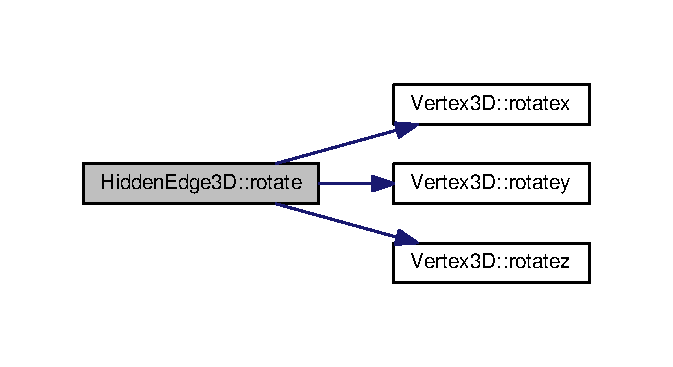
\includegraphics[width=323pt]{class_hidden_edge3_d_a47c13f15de3ae05d2ea539ed094084e9_cgraph}
\end{center}
\end{figure}


\index{Hidden\+Edge3D@{Hidden\+Edge3D}!rotatex@{rotatex}}
\index{rotatex@{rotatex}!Hidden\+Edge3D@{Hidden\+Edge3D}}
\subsubsection[{\texorpdfstring{rotatex(double delta, bool dirdelta)}{rotatex(double delta, bool dirdelta)}}]{\setlength{\rightskip}{0pt plus 5cm}void Hidden\+Edge3\+D\+::rotatex (
\begin{DoxyParamCaption}
\item[{double}]{delta, }
\item[{bool}]{dirdelta}
\end{DoxyParamCaption}
)}\hypertarget{class_hidden_edge3_d_af52b93b4ec291277aaf5c1138068f6db}{}\label{class_hidden_edge3_d_af52b93b4ec291277aaf5c1138068f6db}
\index{Hidden\+Edge3D@{Hidden\+Edge3D}!rotatey@{rotatey}}
\index{rotatey@{rotatey}!Hidden\+Edge3D@{Hidden\+Edge3D}}
\subsubsection[{\texorpdfstring{rotatey(double delta, bool dirdelta)}{rotatey(double delta, bool dirdelta)}}]{\setlength{\rightskip}{0pt plus 5cm}void Hidden\+Edge3\+D\+::rotatey (
\begin{DoxyParamCaption}
\item[{double}]{delta, }
\item[{bool}]{dirdelta}
\end{DoxyParamCaption}
)}\hypertarget{class_hidden_edge3_d_aacf1c6981dc9189b56de6f0920e146ce}{}\label{class_hidden_edge3_d_aacf1c6981dc9189b56de6f0920e146ce}
\index{Hidden\+Edge3D@{Hidden\+Edge3D}!rotatez@{rotatez}}
\index{rotatez@{rotatez}!Hidden\+Edge3D@{Hidden\+Edge3D}}
\subsubsection[{\texorpdfstring{rotatez(double delta, bool dirdelta)}{rotatez(double delta, bool dirdelta)}}]{\setlength{\rightskip}{0pt plus 5cm}void Hidden\+Edge3\+D\+::rotatez (
\begin{DoxyParamCaption}
\item[{double}]{delta, }
\item[{bool}]{dirdelta}
\end{DoxyParamCaption}
)}\hypertarget{class_hidden_edge3_d_acf087a769831355854758b043e9b4bfa}{}\label{class_hidden_edge3_d_acf087a769831355854758b043e9b4bfa}


\subsection{Member Data Documentation}
\index{Hidden\+Edge3D@{Hidden\+Edge3D}!x1@{x1}}
\index{x1@{x1}!Hidden\+Edge3D@{Hidden\+Edge3D}}
\subsubsection[{\texorpdfstring{x1}{x1}}]{\setlength{\rightskip}{0pt plus 5cm}double Hidden\+Edge3\+D\+::x1}\hypertarget{class_hidden_edge3_d_a2427c2c64f2923c487e4a05623ba58bb}{}\label{class_hidden_edge3_d_a2427c2c64f2923c487e4a05623ba58bb}
\index{Hidden\+Edge3D@{Hidden\+Edge3D}!x2@{x2}}
\index{x2@{x2}!Hidden\+Edge3D@{Hidden\+Edge3D}}
\subsubsection[{\texorpdfstring{x2}{x2}}]{\setlength{\rightskip}{0pt plus 5cm}double Hidden\+Edge3\+D\+::x2}\hypertarget{class_hidden_edge3_d_adeba8473617de2da7c6276b8f7806fa0}{}\label{class_hidden_edge3_d_adeba8473617de2da7c6276b8f7806fa0}
\index{Hidden\+Edge3D@{Hidden\+Edge3D}!y1@{y1}}
\index{y1@{y1}!Hidden\+Edge3D@{Hidden\+Edge3D}}
\subsubsection[{\texorpdfstring{y1}{y1}}]{\setlength{\rightskip}{0pt plus 5cm}double Hidden\+Edge3\+D\+::y1}\hypertarget{class_hidden_edge3_d_a40b67744e7d07d47204599c5481f5d2e}{}\label{class_hidden_edge3_d_a40b67744e7d07d47204599c5481f5d2e}
\index{Hidden\+Edge3D@{Hidden\+Edge3D}!y2@{y2}}
\index{y2@{y2}!Hidden\+Edge3D@{Hidden\+Edge3D}}
\subsubsection[{\texorpdfstring{y2}{y2}}]{\setlength{\rightskip}{0pt plus 5cm}double Hidden\+Edge3\+D\+::y2}\hypertarget{class_hidden_edge3_d_ab8a6f5b37b5b208042307a8a1060bd0d}{}\label{class_hidden_edge3_d_ab8a6f5b37b5b208042307a8a1060bd0d}
\index{Hidden\+Edge3D@{Hidden\+Edge3D}!z1@{z1}}
\index{z1@{z1}!Hidden\+Edge3D@{Hidden\+Edge3D}}
\subsubsection[{\texorpdfstring{z1}{z1}}]{\setlength{\rightskip}{0pt plus 5cm}double Hidden\+Edge3\+D\+::z1}\hypertarget{class_hidden_edge3_d_ad8b9d5b2867873171153447a1f75204e}{}\label{class_hidden_edge3_d_ad8b9d5b2867873171153447a1f75204e}
\index{Hidden\+Edge3D@{Hidden\+Edge3D}!z2@{z2}}
\index{z2@{z2}!Hidden\+Edge3D@{Hidden\+Edge3D}}
\subsubsection[{\texorpdfstring{z2}{z2}}]{\setlength{\rightskip}{0pt plus 5cm}double Hidden\+Edge3\+D\+::z2}\hypertarget{class_hidden_edge3_d_a6e4a7847916c1849577b18d5823c5e50}{}\label{class_hidden_edge3_d_a6e4a7847916c1849577b18d5823c5e50}


The documentation for this class was generated from the following files\+:\begin{DoxyCompactItemize}
\item 
C\+O\+P290new/include/\hyperlink{3_d_8h}{3\+D.\+h}\item 
C\+O\+P290new/src/\hyperlink{3_d_8cpp}{3\+D.\+cpp}\end{DoxyCompactItemize}

\hypertarget{class_orthographic_view}{}\section{Orthographic\+View Class Reference}
\label{class_orthographic_view}\index{Orthographic\+View@{Orthographic\+View}}


{\ttfamily \#include $<$2\+D.\+h$>$}

\subsection*{Public Attributes}
\begin{DoxyCompactItemize}
\item 
int \hyperlink{class_orthographic_view_ae9f5b34d51d46495fd507dfa8f0c352b}{view\+\_\+type}
\end{DoxyCompactItemize}


\subsection{Member Data Documentation}
\index{Orthographic\+View@{Orthographic\+View}!view\+\_\+type@{view\+\_\+type}}
\index{view\+\_\+type@{view\+\_\+type}!Orthographic\+View@{Orthographic\+View}}
\subsubsection[{\texorpdfstring{view\+\_\+type}{view_type}}]{\setlength{\rightskip}{0pt plus 5cm}int Orthographic\+View\+::view\+\_\+type}\hypertarget{class_orthographic_view_ae9f5b34d51d46495fd507dfa8f0c352b}{}\label{class_orthographic_view_ae9f5b34d51d46495fd507dfa8f0c352b}


The documentation for this class was generated from the following file\+:\begin{DoxyCompactItemize}
\item 
C\+O\+P290new/include/\hyperlink{2_d_8h}{2\+D.\+h}\end{DoxyCompactItemize}

\hypertarget{class_plane3_d}{}\section{Plane3D Class Reference}
\label{class_plane3_d}\index{Plane3D@{Plane3D}}


{\ttfamily \#include $<$3\+D.\+h$>$}

\subsection*{Public Member Functions}
\begin{DoxyCompactItemize}
\item 
void \hyperlink{class_plane3_d_a72b6c267c304c5765452b963d20b4b8b}{translatex} (float dx)
\item 
void \hyperlink{class_plane3_d_af66b3d101511511e3090fb61e57d0975}{translatey} (float dy)
\item 
void \hyperlink{class_plane3_d_ac6f6330a15fc8b4babca1b9fb97fdf87}{translatez} (float dz)
\item 
void \hyperlink{class_plane3_d_a166c66868aa73a487fad0cbae308c9c6}{rotate} (float delta, float theta, bool dirdelta, bool dirtheta, \hyperlink{class_vertex3_d}{Vertex3D} axis)
\end{DoxyCompactItemize}
\subsection*{Public Attributes}
\begin{DoxyCompactItemize}
\item 
std\+::vector$<$ \hyperlink{class_edge3_d}{Edge3D} $>$ \hyperlink{class_plane3_d_aff30a0d398845f7141692fa5d7493280}{plane}
\end{DoxyCompactItemize}


\subsection{Member Function Documentation}
\index{Plane3D@{Plane3D}!rotate@{rotate}}
\index{rotate@{rotate}!Plane3D@{Plane3D}}
\subsubsection[{\texorpdfstring{rotate(float delta, float theta, bool dirdelta, bool dirtheta, Vertex3\+D axis)}{rotate(float delta, float theta, bool dirdelta, bool dirtheta, Vertex3D axis)}}]{\setlength{\rightskip}{0pt plus 5cm}void Plane3\+D\+::rotate (
\begin{DoxyParamCaption}
\item[{float}]{delta, }
\item[{float}]{theta, }
\item[{bool}]{dirdelta, }
\item[{bool}]{dirtheta, }
\item[{{\bf Vertex3D}}]{axis}
\end{DoxyParamCaption}
)\hspace{0.3cm}{\ttfamily [inline]}}\hypertarget{class_plane3_d_a166c66868aa73a487fad0cbae308c9c6}{}\label{class_plane3_d_a166c66868aa73a487fad0cbae308c9c6}
\index{Plane3D@{Plane3D}!translatex@{translatex}}
\index{translatex@{translatex}!Plane3D@{Plane3D}}
\subsubsection[{\texorpdfstring{translatex(float dx)}{translatex(float dx)}}]{\setlength{\rightskip}{0pt plus 5cm}void Plane3\+D\+::translatex (
\begin{DoxyParamCaption}
\item[{float}]{dx}
\end{DoxyParamCaption}
)\hspace{0.3cm}{\ttfamily [inline]}}\hypertarget{class_plane3_d_a72b6c267c304c5765452b963d20b4b8b}{}\label{class_plane3_d_a72b6c267c304c5765452b963d20b4b8b}
\index{Plane3D@{Plane3D}!translatey@{translatey}}
\index{translatey@{translatey}!Plane3D@{Plane3D}}
\subsubsection[{\texorpdfstring{translatey(float dy)}{translatey(float dy)}}]{\setlength{\rightskip}{0pt plus 5cm}void Plane3\+D\+::translatey (
\begin{DoxyParamCaption}
\item[{float}]{dy}
\end{DoxyParamCaption}
)\hspace{0.3cm}{\ttfamily [inline]}}\hypertarget{class_plane3_d_af66b3d101511511e3090fb61e57d0975}{}\label{class_plane3_d_af66b3d101511511e3090fb61e57d0975}
\index{Plane3D@{Plane3D}!translatez@{translatez}}
\index{translatez@{translatez}!Plane3D@{Plane3D}}
\subsubsection[{\texorpdfstring{translatez(float dz)}{translatez(float dz)}}]{\setlength{\rightskip}{0pt plus 5cm}void Plane3\+D\+::translatez (
\begin{DoxyParamCaption}
\item[{float}]{dz}
\end{DoxyParamCaption}
)\hspace{0.3cm}{\ttfamily [inline]}}\hypertarget{class_plane3_d_ac6f6330a15fc8b4babca1b9fb97fdf87}{}\label{class_plane3_d_ac6f6330a15fc8b4babca1b9fb97fdf87}


\subsection{Member Data Documentation}
\index{Plane3D@{Plane3D}!plane@{plane}}
\index{plane@{plane}!Plane3D@{Plane3D}}
\subsubsection[{\texorpdfstring{plane}{plane}}]{\setlength{\rightskip}{0pt plus 5cm}std\+::vector$<${\bf Edge3D}$>$ Plane3\+D\+::plane}\hypertarget{class_plane3_d_aff30a0d398845f7141692fa5d7493280}{}\label{class_plane3_d_aff30a0d398845f7141692fa5d7493280}


The documentation for this class was generated from the following file\+:\begin{DoxyCompactItemize}
\item 
/home/hp/\+Desktop/\+C\+O\+P290new/\+C\+O\+P290/\hyperlink{3_d_8h}{3\+D.\+h}\end{DoxyCompactItemize}

\hypertarget{class_three_d_body}{}\section{Three\+D\+Body Class Reference}
\label{class_three_d_body}\index{Three\+D\+Body@{Three\+D\+Body}}


{\ttfamily \#include $<$3\+D.\+h$>$}

\subsection*{Public Attributes}
\begin{DoxyCompactItemize}
\item 
std\+::vector$<$ \hyperlink{class_vertex3_d}{Vertex3D} $>$ \hyperlink{class_three_d_body_ae85a9587eced34b16806c2c2f009d208}{v}
\item 
std\+::vector$<$ \hyperlink{class_edge3_d}{Edge3D} $>$ \hyperlink{class_three_d_body_a20054d806b11e6d6ee768231a1ee61d3}{e}
\item 
std\+::vector$<$ \hyperlink{class_plane3_d}{Plane3D} $>$ \hyperlink{class_three_d_body_a871bc38d1590dfb2f076a8ca2def89ad}{p}
\item 
std\+::vector$<$ \hyperlink{class_hidden_edge3_d}{Hidden\+Edge3D} $>$ \hyperlink{class_three_d_body_a89940d00825338f6f685b7522be1d200}{he}
\item 
std\+::vector$<$ \hyperlink{class_visible_edge3_d}{Visible\+Edge3D} $>$ \hyperlink{class_three_d_body_ab35d0ee77c7176e3133a9d3357d173e2}{ve}
\end{DoxyCompactItemize}


\subsection{Member Data Documentation}
\index{Three\+D\+Body@{Three\+D\+Body}!e@{e}}
\index{e@{e}!Three\+D\+Body@{Three\+D\+Body}}
\subsubsection[{\texorpdfstring{e}{e}}]{\setlength{\rightskip}{0pt plus 5cm}std\+::vector$<${\bf Edge3D}$>$ Three\+D\+Body\+::e}\hypertarget{class_three_d_body_a20054d806b11e6d6ee768231a1ee61d3}{}\label{class_three_d_body_a20054d806b11e6d6ee768231a1ee61d3}
\index{Three\+D\+Body@{Three\+D\+Body}!he@{he}}
\index{he@{he}!Three\+D\+Body@{Three\+D\+Body}}
\subsubsection[{\texorpdfstring{he}{he}}]{\setlength{\rightskip}{0pt plus 5cm}std\+::vector$<${\bf Hidden\+Edge3D}$>$ Three\+D\+Body\+::he}\hypertarget{class_three_d_body_a89940d00825338f6f685b7522be1d200}{}\label{class_three_d_body_a89940d00825338f6f685b7522be1d200}
\index{Three\+D\+Body@{Three\+D\+Body}!p@{p}}
\index{p@{p}!Three\+D\+Body@{Three\+D\+Body}}
\subsubsection[{\texorpdfstring{p}{p}}]{\setlength{\rightskip}{0pt plus 5cm}std\+::vector$<${\bf Plane3D}$>$ Three\+D\+Body\+::p}\hypertarget{class_three_d_body_a871bc38d1590dfb2f076a8ca2def89ad}{}\label{class_three_d_body_a871bc38d1590dfb2f076a8ca2def89ad}
\index{Three\+D\+Body@{Three\+D\+Body}!v@{v}}
\index{v@{v}!Three\+D\+Body@{Three\+D\+Body}}
\subsubsection[{\texorpdfstring{v}{v}}]{\setlength{\rightskip}{0pt plus 5cm}std\+::vector$<${\bf Vertex3D}$>$ Three\+D\+Body\+::v}\hypertarget{class_three_d_body_ae85a9587eced34b16806c2c2f009d208}{}\label{class_three_d_body_ae85a9587eced34b16806c2c2f009d208}
\index{Three\+D\+Body@{Three\+D\+Body}!ve@{ve}}
\index{ve@{ve}!Three\+D\+Body@{Three\+D\+Body}}
\subsubsection[{\texorpdfstring{ve}{ve}}]{\setlength{\rightskip}{0pt plus 5cm}std\+::vector$<${\bf Visible\+Edge3D}$>$ Three\+D\+Body\+::ve}\hypertarget{class_three_d_body_ab35d0ee77c7176e3133a9d3357d173e2}{}\label{class_three_d_body_ab35d0ee77c7176e3133a9d3357d173e2}


The documentation for this class was generated from the following file\+:\begin{DoxyCompactItemize}
\item 
/home/hp/\+Desktop/\+C\+O\+P290/\hyperlink{3_d_8h}{3\+D.\+h}\end{DoxyCompactItemize}

\hypertarget{class_two_d_body}{}\section{Two\+D\+Body Class Reference}
\label{class_two_d_body}\index{Two\+D\+Body@{Two\+D\+Body}}


{\ttfamily \#include $<$2\+D.\+h$>$}

\subsection*{Public Attributes}
\begin{DoxyCompactItemize}
\item 
std\+::vector$<$ \hyperlink{class_vertex2_d}{Vertex2D} $>$ \hyperlink{class_two_d_body_a28003130b9cd049b6ab0c750af18a7a0}{v}
\item 
std\+::vector$<$ \hyperlink{class_visible_edge}{Visible\+Edge} $>$ \hyperlink{class_two_d_body_ac7b38febf4667a16f07ff25b35bd818d}{ve}
\item 
std\+::vector$<$ \hyperlink{class_hidden_edge}{Hidden\+Edge} $>$ \hyperlink{class_two_d_body_a4123a65d4e19ad38a33bca38f121d4be}{he}
\item 
std\+::vector$<$ \hyperlink{class_orthographic_view}{Orthographic\+View} $>$ \hyperlink{class_two_d_body_ab3fca58e4b377854805f3149c5e1a96e}{view}
\end{DoxyCompactItemize}


\subsection{Member Data Documentation}
\index{Two\+D\+Body@{Two\+D\+Body}!he@{he}}
\index{he@{he}!Two\+D\+Body@{Two\+D\+Body}}
\subsubsection[{\texorpdfstring{he}{he}}]{\setlength{\rightskip}{0pt plus 5cm}std\+::vector$<${\bf Hidden\+Edge}$>$ Two\+D\+Body\+::he}\hypertarget{class_two_d_body_a4123a65d4e19ad38a33bca38f121d4be}{}\label{class_two_d_body_a4123a65d4e19ad38a33bca38f121d4be}
\index{Two\+D\+Body@{Two\+D\+Body}!v@{v}}
\index{v@{v}!Two\+D\+Body@{Two\+D\+Body}}
\subsubsection[{\texorpdfstring{v}{v}}]{\setlength{\rightskip}{0pt plus 5cm}std\+::vector$<${\bf Vertex2D}$>$ Two\+D\+Body\+::v}\hypertarget{class_two_d_body_a28003130b9cd049b6ab0c750af18a7a0}{}\label{class_two_d_body_a28003130b9cd049b6ab0c750af18a7a0}
\index{Two\+D\+Body@{Two\+D\+Body}!ve@{ve}}
\index{ve@{ve}!Two\+D\+Body@{Two\+D\+Body}}
\subsubsection[{\texorpdfstring{ve}{ve}}]{\setlength{\rightskip}{0pt plus 5cm}std\+::vector$<${\bf Visible\+Edge}$>$ Two\+D\+Body\+::ve}\hypertarget{class_two_d_body_ac7b38febf4667a16f07ff25b35bd818d}{}\label{class_two_d_body_ac7b38febf4667a16f07ff25b35bd818d}
\index{Two\+D\+Body@{Two\+D\+Body}!view@{view}}
\index{view@{view}!Two\+D\+Body@{Two\+D\+Body}}
\subsubsection[{\texorpdfstring{view}{view}}]{\setlength{\rightskip}{0pt plus 5cm}std\+::vector$<${\bf Orthographic\+View}$>$ Two\+D\+Body\+::view}\hypertarget{class_two_d_body_ab3fca58e4b377854805f3149c5e1a96e}{}\label{class_two_d_body_ab3fca58e4b377854805f3149c5e1a96e}


The documentation for this class was generated from the following file\+:\begin{DoxyCompactItemize}
\item 
/home/hp/\+Desktop/\+C\+O\+P290new/\+C\+O\+P290/\hyperlink{2_d_8h}{2\+D.\+h}\end{DoxyCompactItemize}

\hypertarget{class_vertex2_d}{}\section{Vertex2D Class Reference}
\label{class_vertex2_d}\index{Vertex2D@{Vertex2D}}


{\ttfamily \#include $<$2\+D.\+h$>$}

\subsection*{Public Member Functions}
\begin{DoxyCompactItemize}
\item 
void \hyperlink{class_vertex2_d_a609ec788770d068ab270019916abb718}{translatex} (float dx)
\item 
void \hyperlink{class_vertex2_d_a5b03faf3e13190d9cd04e576d9991d88}{translatey} (float dy)
\item 
void \hyperlink{class_vertex2_d_ac89aa0418ca3e0d57ee3352945bd34c9}{rotate} (float delta, bool dirdelta, \hyperlink{class_vertex2_d}{Vertex2D} axis)
\end{DoxyCompactItemize}
\subsection*{Public Attributes}
\begin{DoxyCompactItemize}
\item 
float \hyperlink{class_vertex2_d_a39275a5945c972e573be08b52031a7d4}{x}
\item 
float \hyperlink{class_vertex2_d_ac3948cfb8740e52bfa30daaf17cc5043}{y}
\end{DoxyCompactItemize}


\subsection{Member Function Documentation}
\index{Vertex2D@{Vertex2D}!rotate@{rotate}}
\index{rotate@{rotate}!Vertex2D@{Vertex2D}}
\subsubsection[{\texorpdfstring{rotate(float delta, bool dirdelta, Vertex2\+D axis)}{rotate(float delta, bool dirdelta, Vertex2D axis)}}]{\setlength{\rightskip}{0pt plus 5cm}void Vertex2\+D\+::rotate (
\begin{DoxyParamCaption}
\item[{float}]{delta, }
\item[{bool}]{dirdelta, }
\item[{{\bf Vertex2D}}]{axis}
\end{DoxyParamCaption}
)\hspace{0.3cm}{\ttfamily [inline]}}\hypertarget{class_vertex2_d_ac89aa0418ca3e0d57ee3352945bd34c9}{}\label{class_vertex2_d_ac89aa0418ca3e0d57ee3352945bd34c9}
\index{Vertex2D@{Vertex2D}!translatex@{translatex}}
\index{translatex@{translatex}!Vertex2D@{Vertex2D}}
\subsubsection[{\texorpdfstring{translatex(float dx)}{translatex(float dx)}}]{\setlength{\rightskip}{0pt plus 5cm}void Vertex2\+D\+::translatex (
\begin{DoxyParamCaption}
\item[{float}]{dx}
\end{DoxyParamCaption}
)\hspace{0.3cm}{\ttfamily [inline]}}\hypertarget{class_vertex2_d_a609ec788770d068ab270019916abb718}{}\label{class_vertex2_d_a609ec788770d068ab270019916abb718}
\index{Vertex2D@{Vertex2D}!translatey@{translatey}}
\index{translatey@{translatey}!Vertex2D@{Vertex2D}}
\subsubsection[{\texorpdfstring{translatey(float dy)}{translatey(float dy)}}]{\setlength{\rightskip}{0pt plus 5cm}void Vertex2\+D\+::translatey (
\begin{DoxyParamCaption}
\item[{float}]{dy}
\end{DoxyParamCaption}
)\hspace{0.3cm}{\ttfamily [inline]}}\hypertarget{class_vertex2_d_a5b03faf3e13190d9cd04e576d9991d88}{}\label{class_vertex2_d_a5b03faf3e13190d9cd04e576d9991d88}


\subsection{Member Data Documentation}
\index{Vertex2D@{Vertex2D}!x@{x}}
\index{x@{x}!Vertex2D@{Vertex2D}}
\subsubsection[{\texorpdfstring{x}{x}}]{\setlength{\rightskip}{0pt plus 5cm}float Vertex2\+D\+::x}\hypertarget{class_vertex2_d_a39275a5945c972e573be08b52031a7d4}{}\label{class_vertex2_d_a39275a5945c972e573be08b52031a7d4}
\index{Vertex2D@{Vertex2D}!y@{y}}
\index{y@{y}!Vertex2D@{Vertex2D}}
\subsubsection[{\texorpdfstring{y}{y}}]{\setlength{\rightskip}{0pt plus 5cm}float Vertex2\+D\+::y}\hypertarget{class_vertex2_d_ac3948cfb8740e52bfa30daaf17cc5043}{}\label{class_vertex2_d_ac3948cfb8740e52bfa30daaf17cc5043}


The documentation for this class was generated from the following file\+:\begin{DoxyCompactItemize}
\item 
/home/hp/\+Desktop/\+C\+O\+P290/\hyperlink{2_d_8h}{2\+D.\+h}\end{DoxyCompactItemize}

\hypertarget{class_vertex3_d}{}\section{Vertex3D Class Reference}
\label{class_vertex3_d}\index{Vertex3D@{Vertex3D}}


{\ttfamily \#include $<$3\+D.\+h$>$}

\subsection*{Public Member Functions}
\begin{DoxyCompactItemize}
\item 
void \hyperlink{class_vertex3_d_a55c9e183f88bd026fb4563200f189895}{translatex} (float dx)
\item 
void \hyperlink{class_vertex3_d_afecdb92ffcdc23ceed0772ac9ce42f05}{translatey} (float dy)
\item 
void \hyperlink{class_vertex3_d_a74d4ae70ac0a9cb92e121d7607d42040}{translatez} (float dz)
\item 
void \hyperlink{class_vertex3_d_a3beec96a84611a22956c63b751d1ae40}{rotate} (float delta, float theta, bool dirdelta, bool dirtheta, \hyperlink{class_vertex3_d}{Vertex3D} axis)
\end{DoxyCompactItemize}
\subsection*{Public Attributes}
\begin{DoxyCompactItemize}
\item 
float \hyperlink{class_vertex3_d_a31874fac8de9ea8aa004f7d62c3b0a82}{x}
\item 
float \hyperlink{class_vertex3_d_acc2ceb770e03d6facf4c921de0eaf3d8}{y}
\item 
float \hyperlink{class_vertex3_d_af04a23eeeea792a53123e2d622395f8f}{z}
\end{DoxyCompactItemize}


\subsection{Member Function Documentation}
\index{Vertex3D@{Vertex3D}!rotate@{rotate}}
\index{rotate@{rotate}!Vertex3D@{Vertex3D}}
\subsubsection[{\texorpdfstring{rotate(float delta, float theta, bool dirdelta, bool dirtheta, Vertex3\+D axis)}{rotate(float delta, float theta, bool dirdelta, bool dirtheta, Vertex3D axis)}}]{\setlength{\rightskip}{0pt plus 5cm}void Vertex3\+D\+::rotate (
\begin{DoxyParamCaption}
\item[{float}]{delta, }
\item[{float}]{theta, }
\item[{bool}]{dirdelta, }
\item[{bool}]{dirtheta, }
\item[{{\bf Vertex3D}}]{axis}
\end{DoxyParamCaption}
)\hspace{0.3cm}{\ttfamily [inline]}}\hypertarget{class_vertex3_d_a3beec96a84611a22956c63b751d1ae40}{}\label{class_vertex3_d_a3beec96a84611a22956c63b751d1ae40}
\index{Vertex3D@{Vertex3D}!translatex@{translatex}}
\index{translatex@{translatex}!Vertex3D@{Vertex3D}}
\subsubsection[{\texorpdfstring{translatex(float dx)}{translatex(float dx)}}]{\setlength{\rightskip}{0pt plus 5cm}void Vertex3\+D\+::translatex (
\begin{DoxyParamCaption}
\item[{float}]{dx}
\end{DoxyParamCaption}
)\hspace{0.3cm}{\ttfamily [inline]}}\hypertarget{class_vertex3_d_a55c9e183f88bd026fb4563200f189895}{}\label{class_vertex3_d_a55c9e183f88bd026fb4563200f189895}
\index{Vertex3D@{Vertex3D}!translatey@{translatey}}
\index{translatey@{translatey}!Vertex3D@{Vertex3D}}
\subsubsection[{\texorpdfstring{translatey(float dy)}{translatey(float dy)}}]{\setlength{\rightskip}{0pt plus 5cm}void Vertex3\+D\+::translatey (
\begin{DoxyParamCaption}
\item[{float}]{dy}
\end{DoxyParamCaption}
)\hspace{0.3cm}{\ttfamily [inline]}}\hypertarget{class_vertex3_d_afecdb92ffcdc23ceed0772ac9ce42f05}{}\label{class_vertex3_d_afecdb92ffcdc23ceed0772ac9ce42f05}
\index{Vertex3D@{Vertex3D}!translatez@{translatez}}
\index{translatez@{translatez}!Vertex3D@{Vertex3D}}
\subsubsection[{\texorpdfstring{translatez(float dz)}{translatez(float dz)}}]{\setlength{\rightskip}{0pt plus 5cm}void Vertex3\+D\+::translatez (
\begin{DoxyParamCaption}
\item[{float}]{dz}
\end{DoxyParamCaption}
)\hspace{0.3cm}{\ttfamily [inline]}}\hypertarget{class_vertex3_d_a74d4ae70ac0a9cb92e121d7607d42040}{}\label{class_vertex3_d_a74d4ae70ac0a9cb92e121d7607d42040}


\subsection{Member Data Documentation}
\index{Vertex3D@{Vertex3D}!x@{x}}
\index{x@{x}!Vertex3D@{Vertex3D}}
\subsubsection[{\texorpdfstring{x}{x}}]{\setlength{\rightskip}{0pt plus 5cm}float Vertex3\+D\+::x}\hypertarget{class_vertex3_d_a31874fac8de9ea8aa004f7d62c3b0a82}{}\label{class_vertex3_d_a31874fac8de9ea8aa004f7d62c3b0a82}
\index{Vertex3D@{Vertex3D}!y@{y}}
\index{y@{y}!Vertex3D@{Vertex3D}}
\subsubsection[{\texorpdfstring{y}{y}}]{\setlength{\rightskip}{0pt plus 5cm}float Vertex3\+D\+::y}\hypertarget{class_vertex3_d_acc2ceb770e03d6facf4c921de0eaf3d8}{}\label{class_vertex3_d_acc2ceb770e03d6facf4c921de0eaf3d8}
\index{Vertex3D@{Vertex3D}!z@{z}}
\index{z@{z}!Vertex3D@{Vertex3D}}
\subsubsection[{\texorpdfstring{z}{z}}]{\setlength{\rightskip}{0pt plus 5cm}float Vertex3\+D\+::z}\hypertarget{class_vertex3_d_af04a23eeeea792a53123e2d622395f8f}{}\label{class_vertex3_d_af04a23eeeea792a53123e2d622395f8f}


The documentation for this class was generated from the following file\+:\begin{DoxyCompactItemize}
\item 
/home/hp/\+Desktop/\+C\+O\+P290/\hyperlink{3_d_8h}{3\+D.\+h}\end{DoxyCompactItemize}

\hypertarget{class_visible_edge}{}\section{Visible\+Edge Class Reference}
\label{class_visible_edge}\index{Visible\+Edge@{Visible\+Edge}}


{\ttfamily \#include $<$2\+D.\+h$>$}

\subsection*{Public Member Functions}
\begin{DoxyCompactItemize}
\item 
void \hyperlink{class_visible_edge_a23bff57948310c4245e8861815fb37da}{translatex} (float dx)
\item 
void \hyperlink{class_visible_edge_ad44264fbcda3cd572456f3604fa1fc5d}{translatey} (float dy)
\item 
void \hyperlink{class_visible_edge_acdc2b293c735a19b1f2b8621b3febdb4}{rotate} (float delta, bool dirdelta, \hyperlink{class_vertex2_d}{Vertex2D} axis)
\end{DoxyCompactItemize}
\subsection*{Public Attributes}
\begin{DoxyCompactItemize}
\item 
float \hyperlink{class_visible_edge_a7baae9b2413ae1375d49ff023f272ad3}{x1}
\item 
float \hyperlink{class_visible_edge_ad371a067b7175df3ee9a7672a0f36986}{y1}
\item 
float \hyperlink{class_visible_edge_a6524c696bcd4e189dd393832e95bde4c}{x2}
\item 
float \hyperlink{class_visible_edge_a0e125191d1f182de18ce9dfb35a98d68}{y2}
\end{DoxyCompactItemize}


\subsection{Member Function Documentation}
\index{Visible\+Edge@{Visible\+Edge}!rotate@{rotate}}
\index{rotate@{rotate}!Visible\+Edge@{Visible\+Edge}}
\subsubsection[{\texorpdfstring{rotate(float delta, bool dirdelta, Vertex2\+D axis)}{rotate(float delta, bool dirdelta, Vertex2D axis)}}]{\setlength{\rightskip}{0pt plus 5cm}void Visible\+Edge\+::rotate (
\begin{DoxyParamCaption}
\item[{float}]{delta, }
\item[{bool}]{dirdelta, }
\item[{{\bf Vertex2D}}]{axis}
\end{DoxyParamCaption}
)\hspace{0.3cm}{\ttfamily [inline]}}\hypertarget{class_visible_edge_acdc2b293c735a19b1f2b8621b3febdb4}{}\label{class_visible_edge_acdc2b293c735a19b1f2b8621b3febdb4}
\index{Visible\+Edge@{Visible\+Edge}!translatex@{translatex}}
\index{translatex@{translatex}!Visible\+Edge@{Visible\+Edge}}
\subsubsection[{\texorpdfstring{translatex(float dx)}{translatex(float dx)}}]{\setlength{\rightskip}{0pt plus 5cm}void Visible\+Edge\+::translatex (
\begin{DoxyParamCaption}
\item[{float}]{dx}
\end{DoxyParamCaption}
)\hspace{0.3cm}{\ttfamily [inline]}}\hypertarget{class_visible_edge_a23bff57948310c4245e8861815fb37da}{}\label{class_visible_edge_a23bff57948310c4245e8861815fb37da}
\index{Visible\+Edge@{Visible\+Edge}!translatey@{translatey}}
\index{translatey@{translatey}!Visible\+Edge@{Visible\+Edge}}
\subsubsection[{\texorpdfstring{translatey(float dy)}{translatey(float dy)}}]{\setlength{\rightskip}{0pt plus 5cm}void Visible\+Edge\+::translatey (
\begin{DoxyParamCaption}
\item[{float}]{dy}
\end{DoxyParamCaption}
)\hspace{0.3cm}{\ttfamily [inline]}}\hypertarget{class_visible_edge_ad44264fbcda3cd572456f3604fa1fc5d}{}\label{class_visible_edge_ad44264fbcda3cd572456f3604fa1fc5d}


\subsection{Member Data Documentation}
\index{Visible\+Edge@{Visible\+Edge}!x1@{x1}}
\index{x1@{x1}!Visible\+Edge@{Visible\+Edge}}
\subsubsection[{\texorpdfstring{x1}{x1}}]{\setlength{\rightskip}{0pt plus 5cm}float Visible\+Edge\+::x1}\hypertarget{class_visible_edge_a7baae9b2413ae1375d49ff023f272ad3}{}\label{class_visible_edge_a7baae9b2413ae1375d49ff023f272ad3}
\index{Visible\+Edge@{Visible\+Edge}!x2@{x2}}
\index{x2@{x2}!Visible\+Edge@{Visible\+Edge}}
\subsubsection[{\texorpdfstring{x2}{x2}}]{\setlength{\rightskip}{0pt plus 5cm}float Visible\+Edge\+::x2}\hypertarget{class_visible_edge_a6524c696bcd4e189dd393832e95bde4c}{}\label{class_visible_edge_a6524c696bcd4e189dd393832e95bde4c}
\index{Visible\+Edge@{Visible\+Edge}!y1@{y1}}
\index{y1@{y1}!Visible\+Edge@{Visible\+Edge}}
\subsubsection[{\texorpdfstring{y1}{y1}}]{\setlength{\rightskip}{0pt plus 5cm}float Visible\+Edge\+::y1}\hypertarget{class_visible_edge_ad371a067b7175df3ee9a7672a0f36986}{}\label{class_visible_edge_ad371a067b7175df3ee9a7672a0f36986}
\index{Visible\+Edge@{Visible\+Edge}!y2@{y2}}
\index{y2@{y2}!Visible\+Edge@{Visible\+Edge}}
\subsubsection[{\texorpdfstring{y2}{y2}}]{\setlength{\rightskip}{0pt plus 5cm}float Visible\+Edge\+::y2}\hypertarget{class_visible_edge_a0e125191d1f182de18ce9dfb35a98d68}{}\label{class_visible_edge_a0e125191d1f182de18ce9dfb35a98d68}


The documentation for this class was generated from the following file\+:\begin{DoxyCompactItemize}
\item 
/home/hp/\+Desktop/\+C\+O\+P290new/\+C\+O\+P290/\hyperlink{2_d_8h}{2\+D.\+h}\end{DoxyCompactItemize}

\hypertarget{class_visible_edge3_d}{}\section{Visible\+Edge3D Class Reference}
\label{class_visible_edge3_d}\index{Visible\+Edge3D@{Visible\+Edge3D}}


{\ttfamily \#include $<$3\+D.\+h$>$}

\subsection*{Public Member Functions}
\begin{DoxyCompactItemize}
\item 
void \hyperlink{class_visible_edge3_d_a81ab9194da1a4783822791c724e8a63c}{translatex} (float dx)
\item 
void \hyperlink{class_visible_edge3_d_a48f6254fb4e247392cd261a7f937fc63}{translatey} (float dy)
\item 
void \hyperlink{class_visible_edge3_d_a0948f7df911eba185a8a95caeb468c0d}{translatez} (float dz)
\item 
void \hyperlink{class_visible_edge3_d_a264bd0e3184db14052509d8f19d8b6f8}{rotate} (float delta, float theta, bool dirdelta, bool dirtheta, \hyperlink{class_vertex3_d}{Vertex3D} axis)
\end{DoxyCompactItemize}
\subsection*{Public Attributes}
\begin{DoxyCompactItemize}
\item 
float \hyperlink{class_visible_edge3_d_a241363ce7265575a9119b8f217ec3b11}{x1}
\item 
float \hyperlink{class_visible_edge3_d_a97ccd88f6e8c8f92829940dec525bab6}{y1}
\item 
float \hyperlink{class_visible_edge3_d_ad080d0b1f9c8327bb691f421b8f04e3f}{z1}
\item 
float \hyperlink{class_visible_edge3_d_a75364dcc798d833dd3ade53ddf734055}{x2}
\item 
float \hyperlink{class_visible_edge3_d_a58da80f0733956ed974580a414b84e06}{y2}
\item 
float \hyperlink{class_visible_edge3_d_a90b18a97ee484e34b2dc18cadb2366f7}{z2}
\end{DoxyCompactItemize}


\subsection{Member Function Documentation}
\index{Visible\+Edge3D@{Visible\+Edge3D}!rotate@{rotate}}
\index{rotate@{rotate}!Visible\+Edge3D@{Visible\+Edge3D}}
\subsubsection[{\texorpdfstring{rotate(float delta, float theta, bool dirdelta, bool dirtheta, Vertex3\+D axis)}{rotate(float delta, float theta, bool dirdelta, bool dirtheta, Vertex3D axis)}}]{\setlength{\rightskip}{0pt plus 5cm}void Visible\+Edge3\+D\+::rotate (
\begin{DoxyParamCaption}
\item[{float}]{delta, }
\item[{float}]{theta, }
\item[{bool}]{dirdelta, }
\item[{bool}]{dirtheta, }
\item[{{\bf Vertex3D}}]{axis}
\end{DoxyParamCaption}
)\hspace{0.3cm}{\ttfamily [inline]}}\hypertarget{class_visible_edge3_d_a264bd0e3184db14052509d8f19d8b6f8}{}\label{class_visible_edge3_d_a264bd0e3184db14052509d8f19d8b6f8}
\index{Visible\+Edge3D@{Visible\+Edge3D}!translatex@{translatex}}
\index{translatex@{translatex}!Visible\+Edge3D@{Visible\+Edge3D}}
\subsubsection[{\texorpdfstring{translatex(float dx)}{translatex(float dx)}}]{\setlength{\rightskip}{0pt plus 5cm}void Visible\+Edge3\+D\+::translatex (
\begin{DoxyParamCaption}
\item[{float}]{dx}
\end{DoxyParamCaption}
)\hspace{0.3cm}{\ttfamily [inline]}}\hypertarget{class_visible_edge3_d_a81ab9194da1a4783822791c724e8a63c}{}\label{class_visible_edge3_d_a81ab9194da1a4783822791c724e8a63c}
\index{Visible\+Edge3D@{Visible\+Edge3D}!translatey@{translatey}}
\index{translatey@{translatey}!Visible\+Edge3D@{Visible\+Edge3D}}
\subsubsection[{\texorpdfstring{translatey(float dy)}{translatey(float dy)}}]{\setlength{\rightskip}{0pt plus 5cm}void Visible\+Edge3\+D\+::translatey (
\begin{DoxyParamCaption}
\item[{float}]{dy}
\end{DoxyParamCaption}
)\hspace{0.3cm}{\ttfamily [inline]}}\hypertarget{class_visible_edge3_d_a48f6254fb4e247392cd261a7f937fc63}{}\label{class_visible_edge3_d_a48f6254fb4e247392cd261a7f937fc63}
\index{Visible\+Edge3D@{Visible\+Edge3D}!translatez@{translatez}}
\index{translatez@{translatez}!Visible\+Edge3D@{Visible\+Edge3D}}
\subsubsection[{\texorpdfstring{translatez(float dz)}{translatez(float dz)}}]{\setlength{\rightskip}{0pt plus 5cm}void Visible\+Edge3\+D\+::translatez (
\begin{DoxyParamCaption}
\item[{float}]{dz}
\end{DoxyParamCaption}
)\hspace{0.3cm}{\ttfamily [inline]}}\hypertarget{class_visible_edge3_d_a0948f7df911eba185a8a95caeb468c0d}{}\label{class_visible_edge3_d_a0948f7df911eba185a8a95caeb468c0d}


\subsection{Member Data Documentation}
\index{Visible\+Edge3D@{Visible\+Edge3D}!x1@{x1}}
\index{x1@{x1}!Visible\+Edge3D@{Visible\+Edge3D}}
\subsubsection[{\texorpdfstring{x1}{x1}}]{\setlength{\rightskip}{0pt plus 5cm}float Visible\+Edge3\+D\+::x1}\hypertarget{class_visible_edge3_d_a241363ce7265575a9119b8f217ec3b11}{}\label{class_visible_edge3_d_a241363ce7265575a9119b8f217ec3b11}
\index{Visible\+Edge3D@{Visible\+Edge3D}!x2@{x2}}
\index{x2@{x2}!Visible\+Edge3D@{Visible\+Edge3D}}
\subsubsection[{\texorpdfstring{x2}{x2}}]{\setlength{\rightskip}{0pt plus 5cm}float Visible\+Edge3\+D\+::x2}\hypertarget{class_visible_edge3_d_a75364dcc798d833dd3ade53ddf734055}{}\label{class_visible_edge3_d_a75364dcc798d833dd3ade53ddf734055}
\index{Visible\+Edge3D@{Visible\+Edge3D}!y1@{y1}}
\index{y1@{y1}!Visible\+Edge3D@{Visible\+Edge3D}}
\subsubsection[{\texorpdfstring{y1}{y1}}]{\setlength{\rightskip}{0pt plus 5cm}float Visible\+Edge3\+D\+::y1}\hypertarget{class_visible_edge3_d_a97ccd88f6e8c8f92829940dec525bab6}{}\label{class_visible_edge3_d_a97ccd88f6e8c8f92829940dec525bab6}
\index{Visible\+Edge3D@{Visible\+Edge3D}!y2@{y2}}
\index{y2@{y2}!Visible\+Edge3D@{Visible\+Edge3D}}
\subsubsection[{\texorpdfstring{y2}{y2}}]{\setlength{\rightskip}{0pt plus 5cm}float Visible\+Edge3\+D\+::y2}\hypertarget{class_visible_edge3_d_a58da80f0733956ed974580a414b84e06}{}\label{class_visible_edge3_d_a58da80f0733956ed974580a414b84e06}
\index{Visible\+Edge3D@{Visible\+Edge3D}!z1@{z1}}
\index{z1@{z1}!Visible\+Edge3D@{Visible\+Edge3D}}
\subsubsection[{\texorpdfstring{z1}{z1}}]{\setlength{\rightskip}{0pt plus 5cm}float Visible\+Edge3\+D\+::z1}\hypertarget{class_visible_edge3_d_ad080d0b1f9c8327bb691f421b8f04e3f}{}\label{class_visible_edge3_d_ad080d0b1f9c8327bb691f421b8f04e3f}
\index{Visible\+Edge3D@{Visible\+Edge3D}!z2@{z2}}
\index{z2@{z2}!Visible\+Edge3D@{Visible\+Edge3D}}
\subsubsection[{\texorpdfstring{z2}{z2}}]{\setlength{\rightskip}{0pt plus 5cm}float Visible\+Edge3\+D\+::z2}\hypertarget{class_visible_edge3_d_a90b18a97ee484e34b2dc18cadb2366f7}{}\label{class_visible_edge3_d_a90b18a97ee484e34b2dc18cadb2366f7}


The documentation for this class was generated from the following file\+:\begin{DoxyCompactItemize}
\item 
/home/hp/\+Desktop/\+C\+O\+P290new/\+C\+O\+P290/\hyperlink{3_d_8h}{3\+D.\+h}\end{DoxyCompactItemize}

\chapter{File Documentation}
\hypertarget{2_d_8h}{}\section{/home/hp/\+Desktop/\+C\+O\+P290new/\+C\+O\+P290/2D.h File Reference}
\label{2_d_8h}\index{/home/hp/\+Desktop/\+C\+O\+P290new/\+C\+O\+P290/2\+D.\+h@{/home/hp/\+Desktop/\+C\+O\+P290new/\+C\+O\+P290/2\+D.\+h}}
{\ttfamily \#include $<$vector$>$}\\*
Include dependency graph for 2D.h\+:\nopagebreak
\begin{figure}[H]
\begin{center}
\leavevmode
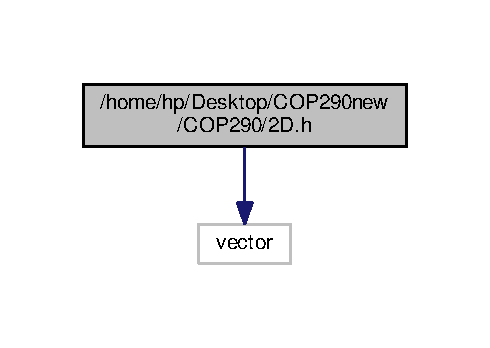
\includegraphics[width=235pt]{2_d_8h__incl}
\end{center}
\end{figure}
This graph shows which files directly or indirectly include this file\+:
\nopagebreak
\begin{figure}[H]
\begin{center}
\leavevmode
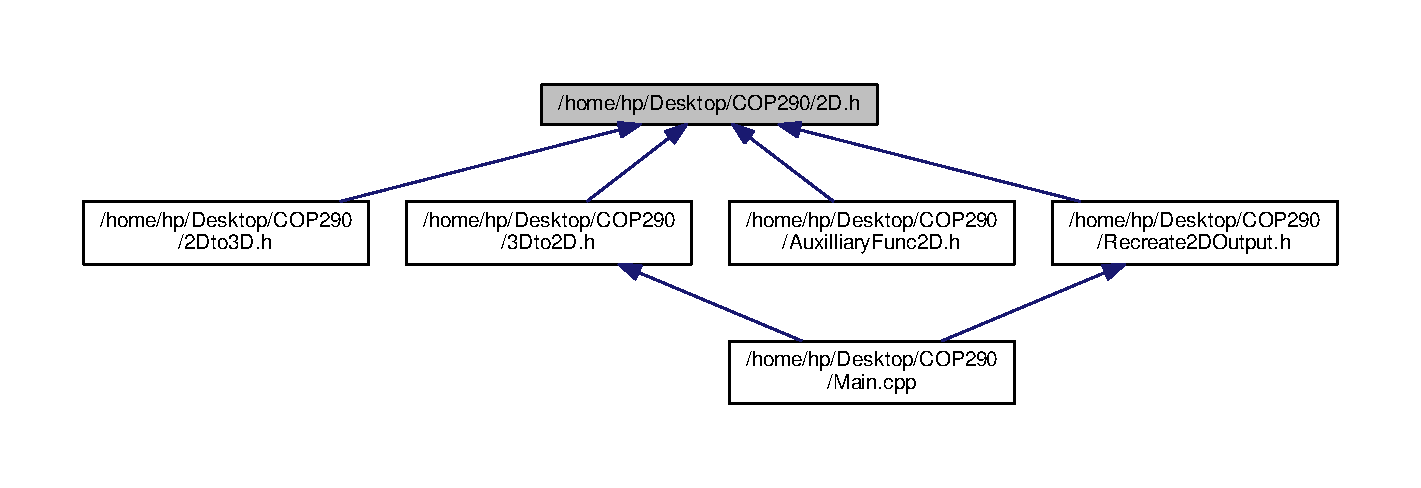
\includegraphics[width=350pt]{2_d_8h__dep__incl}
\end{center}
\end{figure}
\subsection*{Classes}
\begin{DoxyCompactItemize}
\item 
class \hyperlink{class_vertex2_d}{Vertex2D}
\item 
class \hyperlink{class_visible_edge}{Visible\+Edge}
\item 
class \hyperlink{class_orthographic_view}{Orthographic\+View}
\item 
class \hyperlink{class_hidden_edge}{Hidden\+Edge}
\item 
class \hyperlink{class_two_d_body}{Two\+D\+Body}
\end{DoxyCompactItemize}

\hypertarget{2_dto3_d_8h}{}\section{/home/hp/\+Desktop/\+C\+O\+P290/2\+Dto3D.h File Reference}
\label{2_dto3_d_8h}\index{/home/hp/\+Desktop/\+C\+O\+P290/2\+Dto3\+D.\+h@{/home/hp/\+Desktop/\+C\+O\+P290/2\+Dto3\+D.\+h}}
{\ttfamily \#include \char`\"{}3\+D.\+h\char`\"{}}\\*
{\ttfamily \#include \char`\"{}2\+D.\+h\char`\"{}}\\*
{\ttfamily \#include $<$iostream$>$}\\*
{\ttfamily \#include $<$fstream$>$}\\*
{\ttfamily \#include $<$string$>$}\\*
{\ttfamily \#include $<$vector$>$}\\*
Include dependency graph for 2\+Dto3D.h\+:
\nopagebreak
\begin{figure}[H]
\begin{center}
\leavevmode
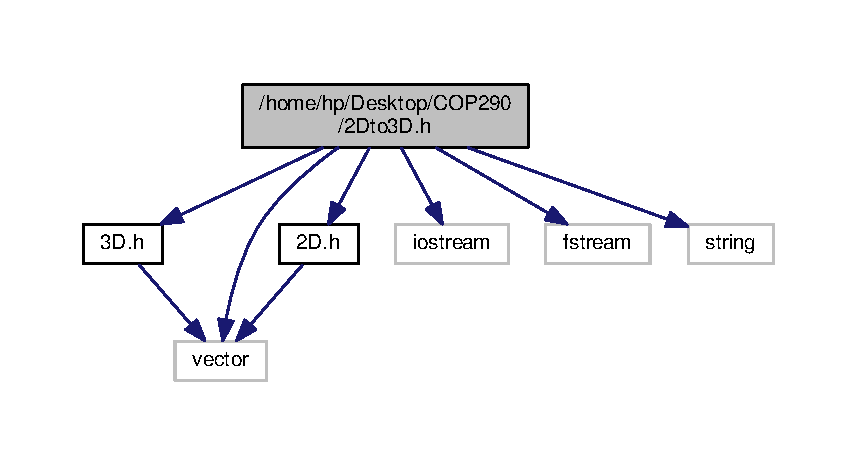
\includegraphics[width=350pt]{2_dto3_d_8h__incl}
\end{center}
\end{figure}
\subsection*{Macros}
\begin{DoxyCompactItemize}
\item 
\#define \hyperlink{2_dto3_d_8h_ac6fd404474b751c083f09311e9d421ac}{O\+D2\+\_\+H}
\end{DoxyCompactItemize}
\subsection*{Functions}
\begin{DoxyCompactItemize}
\item 
std\+::vector$<$ float $>$ \hyperlink{2_dto3_d_8h_a2075cf7d8a5a2b03b220625722bae4b3}{normalofplane} (char $\ast$plane)
\item 
void \hyperlink{2_dto3_d_8h_a776e08df14c4c59ad7d987e9cb1cd812}{viewtype} (\hyperlink{class_two_d_body}{Two\+D\+Body} twodbody)
\item 
void \hyperlink{2_dto3_d_8h_af0b2f2ff42232b5e6978d976cff35455}{topological\+Representation} (\hyperlink{class_two_d_body}{Two\+D\+Body} twodbody)
\item 
void \hyperlink{2_dto3_d_8h_a424d19e29f567e291bb3a272a2607258}{three\+D\+Reconstruct} (\hyperlink{class_two_d_body}{Two\+D\+Body} twodbody, Threebody threebody)
\end{DoxyCompactItemize}


\subsection{Macro Definition Documentation}
\index{2\+Dto3\+D.\+h@{2\+Dto3\+D.\+h}!O\+D2\+\_\+H@{O\+D2\+\_\+H}}
\index{O\+D2\+\_\+H@{O\+D2\+\_\+H}!2\+Dto3\+D.\+h@{2\+Dto3\+D.\+h}}
\subsubsection[{\texorpdfstring{O\+D2\+\_\+H}{OD2_H}}]{\setlength{\rightskip}{0pt plus 5cm}\#define O\+D2\+\_\+H}\hypertarget{2_dto3_d_8h_ac6fd404474b751c083f09311e9d421ac}{}\label{2_dto3_d_8h_ac6fd404474b751c083f09311e9d421ac}


\subsection{Function Documentation}
\index{2\+Dto3\+D.\+h@{2\+Dto3\+D.\+h}!normalofplane@{normalofplane}}
\index{normalofplane@{normalofplane}!2\+Dto3\+D.\+h@{2\+Dto3\+D.\+h}}
\subsubsection[{\texorpdfstring{normalofplane(char $\ast$plane)}{normalofplane(char *plane)}}]{\setlength{\rightskip}{0pt plus 5cm}std\+::vector$<$float$>$ normalofplane (
\begin{DoxyParamCaption}
\item[{char $\ast$}]{plane}
\end{DoxyParamCaption}
)}\hypertarget{2_dto3_d_8h_a2075cf7d8a5a2b03b220625722bae4b3}{}\label{2_dto3_d_8h_a2075cf7d8a5a2b03b220625722bae4b3}
\index{2\+Dto3\+D.\+h@{2\+Dto3\+D.\+h}!three\+D\+Reconstruct@{three\+D\+Reconstruct}}
\index{three\+D\+Reconstruct@{three\+D\+Reconstruct}!2\+Dto3\+D.\+h@{2\+Dto3\+D.\+h}}
\subsubsection[{\texorpdfstring{three\+D\+Reconstruct(\+Two\+D\+Body twodbody, Threebody threebody)}{threeDReconstruct(TwoDBody twodbody, Threebody threebody)}}]{\setlength{\rightskip}{0pt plus 5cm}void three\+D\+Reconstruct (
\begin{DoxyParamCaption}
\item[{{\bf Two\+D\+Body}}]{twodbody, }
\item[{Threebody}]{threebody}
\end{DoxyParamCaption}
)}\hypertarget{2_dto3_d_8h_a424d19e29f567e291bb3a272a2607258}{}\label{2_dto3_d_8h_a424d19e29f567e291bb3a272a2607258}
\index{2\+Dto3\+D.\+h@{2\+Dto3\+D.\+h}!topological\+Representation@{topological\+Representation}}
\index{topological\+Representation@{topological\+Representation}!2\+Dto3\+D.\+h@{2\+Dto3\+D.\+h}}
\subsubsection[{\texorpdfstring{topological\+Representation(\+Two\+D\+Body twodbody)}{topologicalRepresentation(TwoDBody twodbody)}}]{\setlength{\rightskip}{0pt plus 5cm}void topological\+Representation (
\begin{DoxyParamCaption}
\item[{{\bf Two\+D\+Body}}]{twodbody}
\end{DoxyParamCaption}
)}\hypertarget{2_dto3_d_8h_af0b2f2ff42232b5e6978d976cff35455}{}\label{2_dto3_d_8h_af0b2f2ff42232b5e6978d976cff35455}
\index{2\+Dto3\+D.\+h@{2\+Dto3\+D.\+h}!viewtype@{viewtype}}
\index{viewtype@{viewtype}!2\+Dto3\+D.\+h@{2\+Dto3\+D.\+h}}
\subsubsection[{\texorpdfstring{viewtype(\+Two\+D\+Body twodbody)}{viewtype(TwoDBody twodbody)}}]{\setlength{\rightskip}{0pt plus 5cm}void viewtype (
\begin{DoxyParamCaption}
\item[{{\bf Two\+D\+Body}}]{twodbody}
\end{DoxyParamCaption}
)}\hypertarget{2_dto3_d_8h_a776e08df14c4c59ad7d987e9cb1cd812}{}\label{2_dto3_d_8h_a776e08df14c4c59ad7d987e9cb1cd812}

\hypertarget{3_d_8h}{}\section{/home/hp/\+Desktop/\+C\+O\+P290/3D.h File Reference}
\label{3_d_8h}\index{/home/hp/\+Desktop/\+C\+O\+P290/3\+D.\+h@{/home/hp/\+Desktop/\+C\+O\+P290/3\+D.\+h}}
{\ttfamily \#include $<$vector$>$}\\*
Include dependency graph for 3D.h\+:
\nopagebreak
\begin{figure}[H]
\begin{center}
\leavevmode
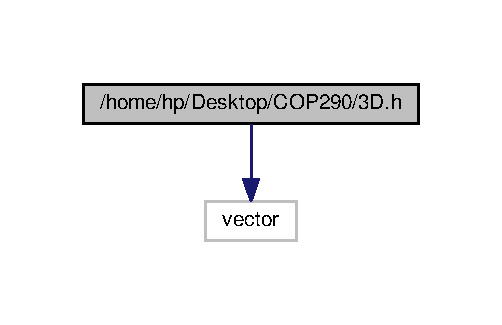
\includegraphics[width=241pt]{3_d_8h__incl}
\end{center}
\end{figure}
This graph shows which files directly or indirectly include this file\+:
\nopagebreak
\begin{figure}[H]
\begin{center}
\leavevmode
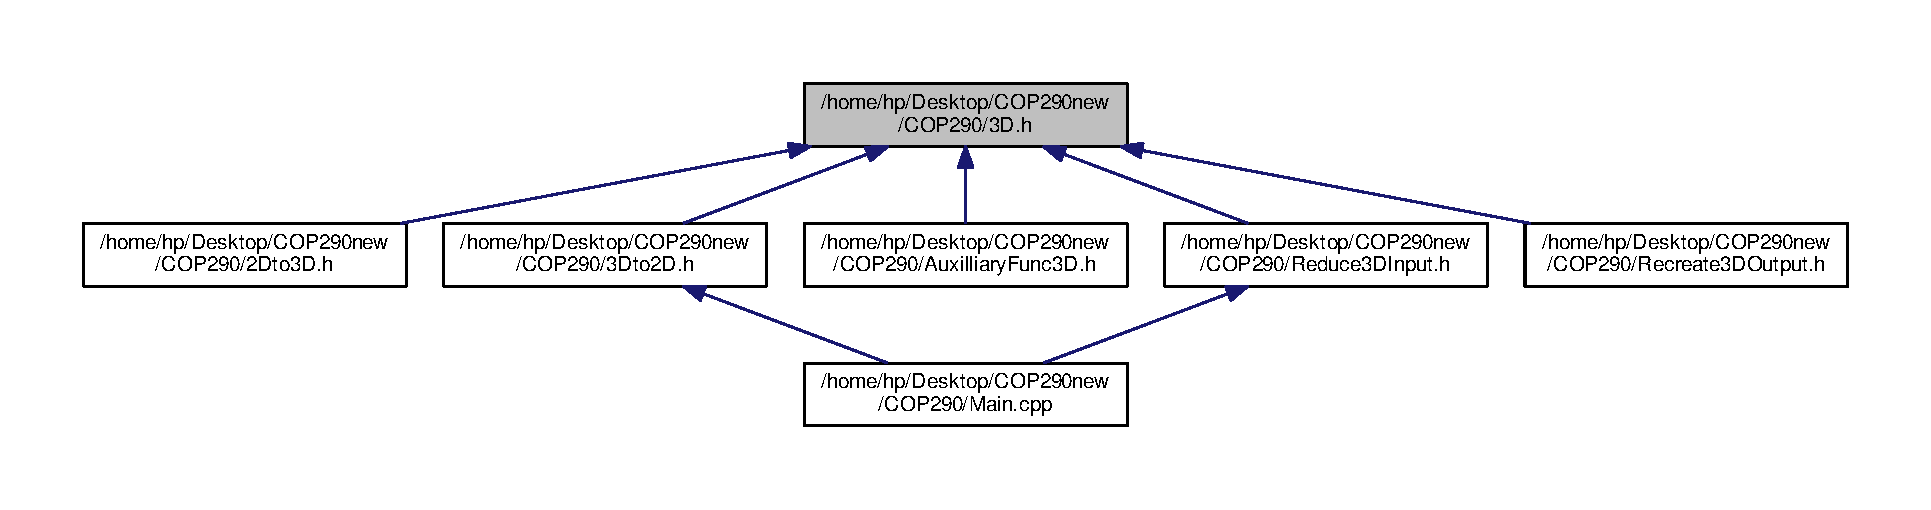
\includegraphics[width=350pt]{3_d_8h__dep__incl}
\end{center}
\end{figure}
\subsection*{Classes}
\begin{DoxyCompactItemize}
\item 
class \hyperlink{class_vertex3_d}{Vertex3D}
\item 
class \hyperlink{class_edge3_d}{Edge3D}
\item 
class \hyperlink{class_plane3_d}{Plane3D}
\item 
class \hyperlink{class_hidden_edge3_d}{Hidden\+Edge3D}
\item 
class \hyperlink{class_visible_edge3_d}{Visible\+Edge3D}
\item 
class \hyperlink{class_three_d_body}{Three\+D\+Body}
\end{DoxyCompactItemize}

\hypertarget{3_dto2_d_8h}{}\section{/home/hp/\+Desktop/\+C\+O\+P290new/\+C\+O\+P290/3\+Dto2D.h File Reference}
\label{3_dto2_d_8h}\index{/home/hp/\+Desktop/\+C\+O\+P290new/\+C\+O\+P290/3\+Dto2\+D.\+h@{/home/hp/\+Desktop/\+C\+O\+P290new/\+C\+O\+P290/3\+Dto2\+D.\+h}}
{\ttfamily \#include \char`\"{}3\+D.\+h\char`\"{}}\\*
{\ttfamily \#include \char`\"{}2\+D.\+h\char`\"{}}\\*
{\ttfamily \#include $<$iostream$>$}\\*
{\ttfamily \#include $<$fstream$>$}\\*
{\ttfamily \#include $<$string$>$}\\*
{\ttfamily \#include $<$vector$>$}\\*
Include dependency graph for 3\+Dto2D.h\+:\nopagebreak
\begin{figure}[H]
\begin{center}
\leavevmode
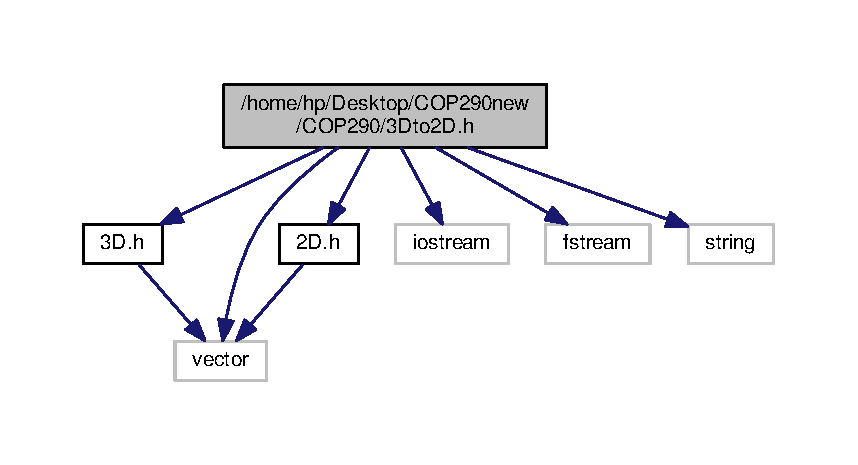
\includegraphics[width=350pt]{3_dto2_d_8h__incl}
\end{center}
\end{figure}
This graph shows which files directly or indirectly include this file\+:\nopagebreak
\begin{figure}[H]
\begin{center}
\leavevmode
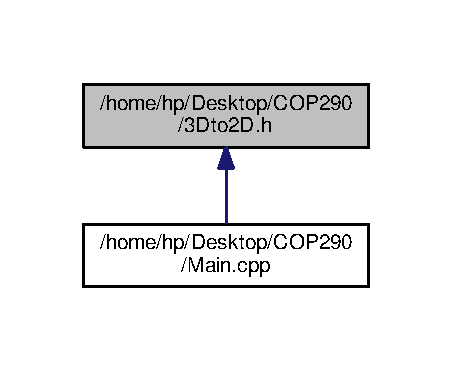
\includegraphics[width=235pt]{3_dto2_d_8h__dep__incl}
\end{center}
\end{figure}
\subsection*{Macros}
\begin{DoxyCompactItemize}
\item 
\#define \hyperlink{3_dto2_d_8h_ac6fd404474b751c083f09311e9d421ac}{O\+D2\+\_\+H}
\end{DoxyCompactItemize}
\subsection*{Functions}
\begin{DoxyCompactItemize}
\item 
std\+::vector$<$ float $>$ \hyperlink{3_dto2_d_8h_a2075cf7d8a5a2b03b220625722bae4b3}{normalofplane} (char $\ast$plane)
\item 
void \hyperlink{3_dto2_d_8h_a9e1f994f69503bda7909e8a017c17b3c}{rotate3D} (\hyperlink{class_three_d_body}{Three\+D\+Body} threedbody, std\+::vector$<$ float $>$ normal, std\+::vector$<$ char $>$ plane)
\item 
void \hyperlink{3_dto2_d_8h_a6aa5b86a823784b89de44bee6a057b7a}{hiddenedgedetection} (\hyperlink{class_three_d_body}{Three\+D\+Body} threedbody, std\+::vector$<$ char $>$ plane)
\item 
\hyperlink{class_two_d_body}{Two\+D\+Body} \hyperlink{3_dto2_d_8h_adda06f7fdd657e0b2430b637007df3a8}{Top\+View} (\hyperlink{class_three_d_body}{Three\+D\+Body} threedbody)
\end{DoxyCompactItemize}


\subsection{Macro Definition Documentation}
\index{3\+Dto2\+D.\+h@{3\+Dto2\+D.\+h}!O\+D2\+\_\+H@{O\+D2\+\_\+H}}
\index{O\+D2\+\_\+H@{O\+D2\+\_\+H}!3\+Dto2\+D.\+h@{3\+Dto2\+D.\+h}}
\subsubsection[{\texorpdfstring{O\+D2\+\_\+H}{OD2_H}}]{\setlength{\rightskip}{0pt plus 5cm}\#define O\+D2\+\_\+H}\hypertarget{3_dto2_d_8h_ac6fd404474b751c083f09311e9d421ac}{}\label{3_dto2_d_8h_ac6fd404474b751c083f09311e9d421ac}


\subsection{Function Documentation}
\index{3\+Dto2\+D.\+h@{3\+Dto2\+D.\+h}!hiddenedgedetection@{hiddenedgedetection}}
\index{hiddenedgedetection@{hiddenedgedetection}!3\+Dto2\+D.\+h@{3\+Dto2\+D.\+h}}
\subsubsection[{\texorpdfstring{hiddenedgedetection(\+Three\+D\+Body threedbody, std\+::vector$<$ char $>$ plane)}{hiddenedgedetection(ThreeDBody threedbody, std::vector< char > plane)}}]{\setlength{\rightskip}{0pt plus 5cm}void hiddenedgedetection (
\begin{DoxyParamCaption}
\item[{{\bf Three\+D\+Body}}]{threedbody, }
\item[{std\+::vector$<$ char $>$}]{plane}
\end{DoxyParamCaption}
)}\hypertarget{3_dto2_d_8h_a6aa5b86a823784b89de44bee6a057b7a}{}\label{3_dto2_d_8h_a6aa5b86a823784b89de44bee6a057b7a}
\index{3\+Dto2\+D.\+h@{3\+Dto2\+D.\+h}!normalofplane@{normalofplane}}
\index{normalofplane@{normalofplane}!3\+Dto2\+D.\+h@{3\+Dto2\+D.\+h}}
\subsubsection[{\texorpdfstring{normalofplane(char $\ast$plane)}{normalofplane(char *plane)}}]{\setlength{\rightskip}{0pt plus 5cm}std\+::vector$<$float$>$ normalofplane (
\begin{DoxyParamCaption}
\item[{char $\ast$}]{plane}
\end{DoxyParamCaption}
)}\hypertarget{3_dto2_d_8h_a2075cf7d8a5a2b03b220625722bae4b3}{}\label{3_dto2_d_8h_a2075cf7d8a5a2b03b220625722bae4b3}
\index{3\+Dto2\+D.\+h@{3\+Dto2\+D.\+h}!rotate3D@{rotate3D}}
\index{rotate3D@{rotate3D}!3\+Dto2\+D.\+h@{3\+Dto2\+D.\+h}}
\subsubsection[{\texorpdfstring{rotate3\+D(\+Three\+D\+Body threedbody, std\+::vector$<$ float $>$ normal, std\+::vector$<$ char $>$ plane)}{rotate3D(ThreeDBody threedbody, std::vector< float > normal, std::vector< char > plane)}}]{\setlength{\rightskip}{0pt plus 5cm}void rotate3D (
\begin{DoxyParamCaption}
\item[{{\bf Three\+D\+Body}}]{threedbody, }
\item[{std\+::vector$<$ float $>$}]{normal, }
\item[{std\+::vector$<$ char $>$}]{plane}
\end{DoxyParamCaption}
)}\hypertarget{3_dto2_d_8h_a9e1f994f69503bda7909e8a017c17b3c}{}\label{3_dto2_d_8h_a9e1f994f69503bda7909e8a017c17b3c}
\index{3\+Dto2\+D.\+h@{3\+Dto2\+D.\+h}!Top\+View@{Top\+View}}
\index{Top\+View@{Top\+View}!3\+Dto2\+D.\+h@{3\+Dto2\+D.\+h}}
\subsubsection[{\texorpdfstring{Top\+View(\+Three\+D\+Body threedbody)}{TopView(ThreeDBody threedbody)}}]{\setlength{\rightskip}{0pt plus 5cm}{\bf Two\+D\+Body} Top\+View (
\begin{DoxyParamCaption}
\item[{{\bf Three\+D\+Body}}]{threedbody}
\end{DoxyParamCaption}
)}\hypertarget{3_dto2_d_8h_adda06f7fdd657e0b2430b637007df3a8}{}\label{3_dto2_d_8h_adda06f7fdd657e0b2430b637007df3a8}

\hypertarget{_auxilliary_func2_d_8h}{}\section{/home/hp/\+Desktop/\+C\+O\+P290/\+Auxilliary\+Func2D.h File Reference}
\label{_auxilliary_func2_d_8h}\index{/home/hp/\+Desktop/\+C\+O\+P290/\+Auxilliary\+Func2\+D.\+h@{/home/hp/\+Desktop/\+C\+O\+P290/\+Auxilliary\+Func2\+D.\+h}}
{\ttfamily \#include \char`\"{}2\+D.\+h\char`\"{}}\\*
Include dependency graph for Auxilliary\+Func2\+D.\+h\+:
\nopagebreak
\begin{figure}[H]
\begin{center}
\leavevmode
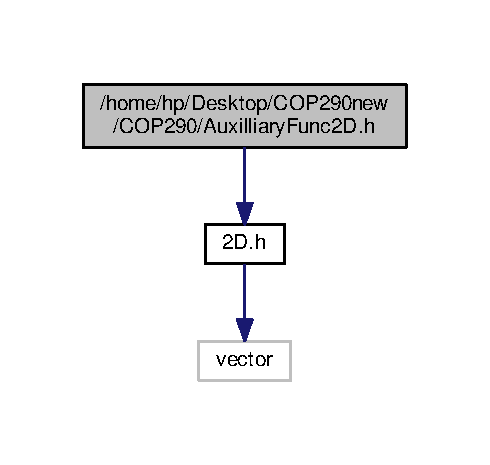
\includegraphics[width=217pt]{_auxilliary_func2_d_8h__incl}
\end{center}
\end{figure}
\subsection*{Functions}
\begin{DoxyCompactItemize}
\item 
void \hyperlink{_auxilliary_func2_d_8h_a3a67c3e0d21d8da67eb292f69aff7ba2}{translate2D} (float dx, float dy, \hyperlink{class_two_d_body}{Two\+D\+Body} twobody)
\item 
void \hyperlink{_auxilliary_func2_d_8h_ab2eb7b02d456077c961cda0961a2618c}{rotate2D} (float delta, float theta, bool dirdelta, Vertex axis)
\item 
void \hyperlink{_auxilliary_func2_d_8h_ae40354fc7ce7198ef8ae37e21b3df90d}{viewtype} (int x, int y)
\end{DoxyCompactItemize}


\subsection{Function Documentation}
\index{Auxilliary\+Func2\+D.\+h@{Auxilliary\+Func2\+D.\+h}!rotate2D@{rotate2D}}
\index{rotate2D@{rotate2D}!Auxilliary\+Func2\+D.\+h@{Auxilliary\+Func2\+D.\+h}}
\subsubsection[{\texorpdfstring{rotate2\+D(float delta, float theta, bool dirdelta, Vertex axis)}{rotate2D(float delta, float theta, bool dirdelta, Vertex axis)}}]{\setlength{\rightskip}{0pt plus 5cm}void rotate2D (
\begin{DoxyParamCaption}
\item[{float}]{delta, }
\item[{float}]{theta, }
\item[{bool}]{dirdelta, }
\item[{Vertex}]{axis}
\end{DoxyParamCaption}
)}\hypertarget{_auxilliary_func2_d_8h_ab2eb7b02d456077c961cda0961a2618c}{}\label{_auxilliary_func2_d_8h_ab2eb7b02d456077c961cda0961a2618c}
\index{Auxilliary\+Func2\+D.\+h@{Auxilliary\+Func2\+D.\+h}!translate2D@{translate2D}}
\index{translate2D@{translate2D}!Auxilliary\+Func2\+D.\+h@{Auxilliary\+Func2\+D.\+h}}
\subsubsection[{\texorpdfstring{translate2\+D(float dx, float dy, Two\+D\+Body twobody)}{translate2D(float dx, float dy, TwoDBody twobody)}}]{\setlength{\rightskip}{0pt plus 5cm}void translate2D (
\begin{DoxyParamCaption}
\item[{float}]{dx, }
\item[{float}]{dy, }
\item[{{\bf Two\+D\+Body}}]{twobody}
\end{DoxyParamCaption}
)}\hypertarget{_auxilliary_func2_d_8h_a3a67c3e0d21d8da67eb292f69aff7ba2}{}\label{_auxilliary_func2_d_8h_a3a67c3e0d21d8da67eb292f69aff7ba2}
\index{Auxilliary\+Func2\+D.\+h@{Auxilliary\+Func2\+D.\+h}!viewtype@{viewtype}}
\index{viewtype@{viewtype}!Auxilliary\+Func2\+D.\+h@{Auxilliary\+Func2\+D.\+h}}
\subsubsection[{\texorpdfstring{viewtype(int x, int y)}{viewtype(int x, int y)}}]{\setlength{\rightskip}{0pt plus 5cm}void viewtype (
\begin{DoxyParamCaption}
\item[{int}]{x, }
\item[{int}]{y}
\end{DoxyParamCaption}
)}\hypertarget{_auxilliary_func2_d_8h_ae40354fc7ce7198ef8ae37e21b3df90d}{}\label{_auxilliary_func2_d_8h_ae40354fc7ce7198ef8ae37e21b3df90d}

\hypertarget{_auxilliary_func3_d_8h}{}\section{/home/hp/\+Desktop/\+C\+O\+P290new/\+C\+O\+P290/\+Auxilliary\+Func3D.h File Reference}
\label{_auxilliary_func3_d_8h}\index{/home/hp/\+Desktop/\+C\+O\+P290new/\+C\+O\+P290/\+Auxilliary\+Func3\+D.\+h@{/home/hp/\+Desktop/\+C\+O\+P290new/\+C\+O\+P290/\+Auxilliary\+Func3\+D.\+h}}
{\ttfamily \#include \char`\"{}3\+D.\+h\char`\"{}}\\*
Include dependency graph for Auxilliary\+Func3\+D.\+h\+:\nopagebreak
\begin{figure}[H]
\begin{center}
\leavevmode
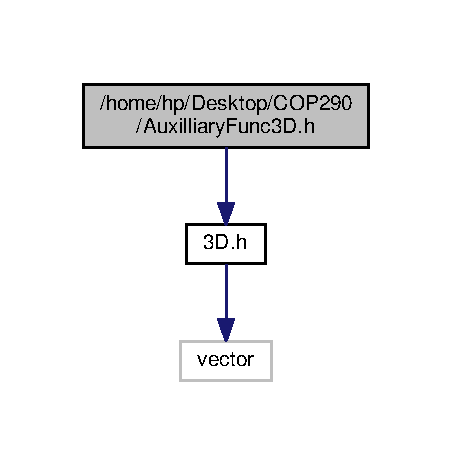
\includegraphics[width=235pt]{_auxilliary_func3_d_8h__incl}
\end{center}
\end{figure}
\subsection*{Functions}
\begin{DoxyCompactItemize}
\item 
void \hyperlink{_auxilliary_func3_d_8h_ad625950bb554569a4705664a71eda102}{translate3D} (float dx, float dy, float dz, \hyperlink{class_three_d_body}{Three\+D\+Body} threedbody)
\item 
void \hyperlink{_auxilliary_func3_d_8h_aabeb09a68c6c2b9a285b47f918675c62}{rotate3D} (float delta, float theta, bool dirdelta, bool dirtheta, \hyperlink{class_vertex3_d}{Vertex3D} axis)
\end{DoxyCompactItemize}


\subsection{Function Documentation}
\index{Auxilliary\+Func3\+D.\+h@{Auxilliary\+Func3\+D.\+h}!rotate3D@{rotate3D}}
\index{rotate3D@{rotate3D}!Auxilliary\+Func3\+D.\+h@{Auxilliary\+Func3\+D.\+h}}
\subsubsection[{\texorpdfstring{rotate3\+D(float delta, float theta, bool dirdelta, bool dirtheta, Vertex3\+D axis)}{rotate3D(float delta, float theta, bool dirdelta, bool dirtheta, Vertex3D axis)}}]{\setlength{\rightskip}{0pt plus 5cm}void rotate3D (
\begin{DoxyParamCaption}
\item[{float}]{delta, }
\item[{float}]{theta, }
\item[{bool}]{dirdelta, }
\item[{bool}]{dirtheta, }
\item[{{\bf Vertex3D}}]{axis}
\end{DoxyParamCaption}
)}\hypertarget{_auxilliary_func3_d_8h_aabeb09a68c6c2b9a285b47f918675c62}{}\label{_auxilliary_func3_d_8h_aabeb09a68c6c2b9a285b47f918675c62}
\index{Auxilliary\+Func3\+D.\+h@{Auxilliary\+Func3\+D.\+h}!translate3D@{translate3D}}
\index{translate3D@{translate3D}!Auxilliary\+Func3\+D.\+h@{Auxilliary\+Func3\+D.\+h}}
\subsubsection[{\texorpdfstring{translate3\+D(float dx, float dy, float dz, Three\+D\+Body threedbody)}{translate3D(float dx, float dy, float dz, ThreeDBody threedbody)}}]{\setlength{\rightskip}{0pt plus 5cm}void translate3D (
\begin{DoxyParamCaption}
\item[{float}]{dx, }
\item[{float}]{dy, }
\item[{float}]{dz, }
\item[{{\bf Three\+D\+Body}}]{threedbody}
\end{DoxyParamCaption}
)}\hypertarget{_auxilliary_func3_d_8h_ad625950bb554569a4705664a71eda102}{}\label{_auxilliary_func3_d_8h_ad625950bb554569a4705664a71eda102}

\hypertarget{_main_8cpp}{}\section{/home/hp/\+Desktop/\+C\+O\+P290/\+Main.cpp File Reference}
\label{_main_8cpp}\index{/home/hp/\+Desktop/\+C\+O\+P290/\+Main.\+cpp@{/home/hp/\+Desktop/\+C\+O\+P290/\+Main.\+cpp}}
{\ttfamily \#include \char`\"{}Reduce3\+D\+Input.\+h\char`\"{}}\\*
{\ttfamily \#include \char`\"{}3\+Dto2\+D.\+h\char`\"{}}\\*
{\ttfamily \#include \char`\"{}Recreate2\+D\+Output.\+h\char`\"{}}\\*
Include dependency graph for Main.\+cpp\+:
\nopagebreak
\begin{figure}[H]
\begin{center}
\leavevmode
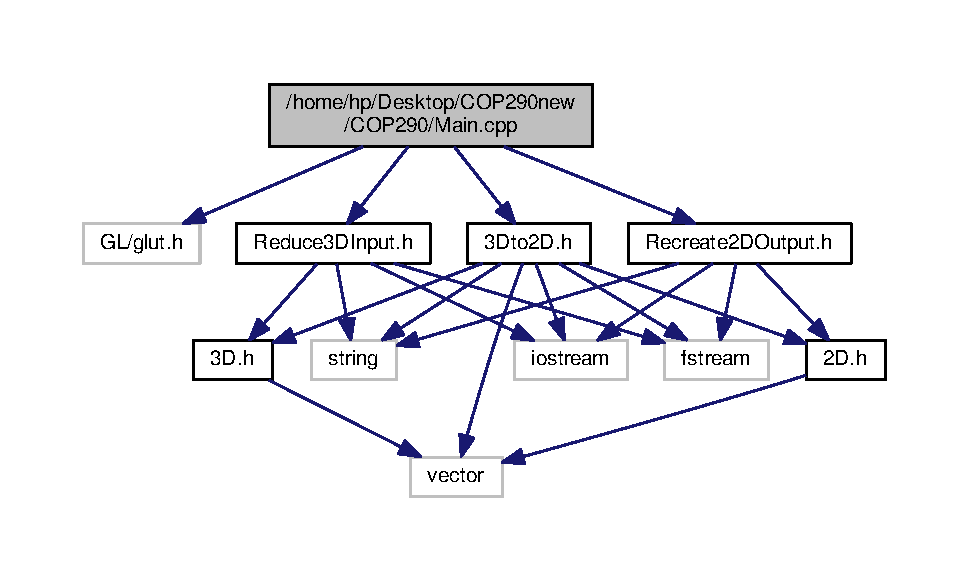
\includegraphics[width=350pt]{_main_8cpp__incl}
\end{center}
\end{figure}
\subsection*{Functions}
\begin{DoxyCompactItemize}
\item 
void \hyperlink{_main_8cpp_a0680a922e25d3366b6ab7396aabe4a49}{Three\+Dto\+TwoD} (std\+::ifstream \&Input\+File)
\end{DoxyCompactItemize}


\subsection{Function Documentation}
\index{Main.\+cpp@{Main.\+cpp}!Three\+Dto\+TwoD@{Three\+Dto\+TwoD}}
\index{Three\+Dto\+TwoD@{Three\+Dto\+TwoD}!Main.\+cpp@{Main.\+cpp}}
\subsubsection[{\texorpdfstring{Three\+Dto\+Two\+D(std\+::ifstream \&\+Input\+File)}{ThreeDtoTwoD(std::ifstream &InputFile)}}]{\setlength{\rightskip}{0pt plus 5cm}void Three\+Dto\+TwoD (
\begin{DoxyParamCaption}
\item[{std\+::ifstream \&}]{Input\+File}
\end{DoxyParamCaption}
)}\hypertarget{_main_8cpp_a0680a922e25d3366b6ab7396aabe4a49}{}\label{_main_8cpp_a0680a922e25d3366b6ab7396aabe4a49}

\hypertarget{_recreate2_d_output_8h}{}\section{/home/hp/\+Desktop/\+C\+O\+P290/\+Recreate2\+D\+Output.h File Reference}
\label{_recreate2_d_output_8h}\index{/home/hp/\+Desktop/\+C\+O\+P290/\+Recreate2\+D\+Output.\+h@{/home/hp/\+Desktop/\+C\+O\+P290/\+Recreate2\+D\+Output.\+h}}
{\ttfamily \#include $<$iostream$>$}\\*
{\ttfamily \#include $<$fstream$>$}\\*
{\ttfamily \#include $<$string$>$}\\*
{\ttfamily \#include \char`\"{}2\+D.\+h\char`\"{}}\\*
Include dependency graph for Recreate2\+D\+Output.\+h\+:
\nopagebreak
\begin{figure}[H]
\begin{center}
\leavevmode
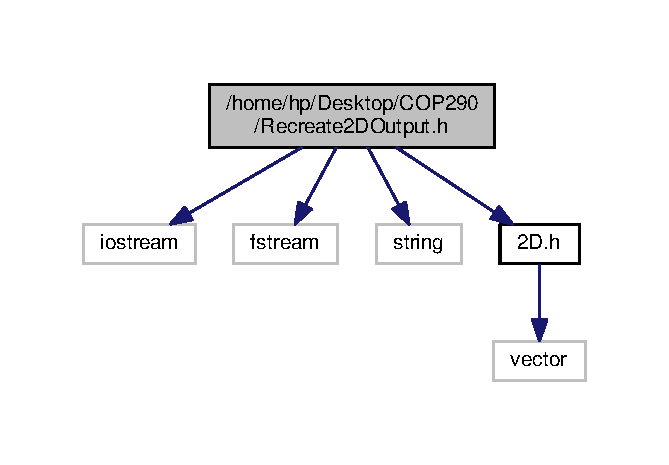
\includegraphics[width=321pt]{_recreate2_d_output_8h__incl}
\end{center}
\end{figure}
This graph shows which files directly or indirectly include this file\+:
\nopagebreak
\begin{figure}[H]
\begin{center}
\leavevmode
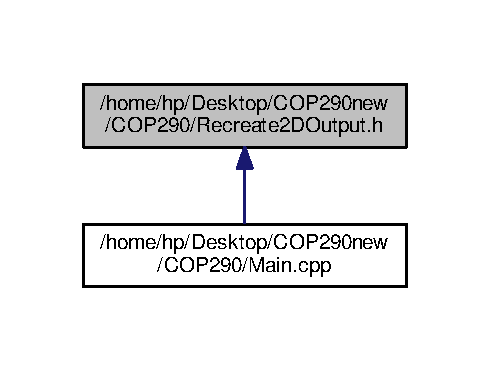
\includegraphics[width=217pt]{_recreate2_d_output_8h__dep__incl}
\end{center}
\end{figure}
\subsection*{Functions}
\begin{DoxyCompactItemize}
\item 
void \hyperlink{_recreate2_d_output_8h_ab29c320ce81f16e12a41dc47a051be9d}{recreate2D} (\hyperlink{class_two_d_body}{Two\+D\+Body} twodbody)
\end{DoxyCompactItemize}


\subsection{Function Documentation}
\index{Recreate2\+D\+Output.\+h@{Recreate2\+D\+Output.\+h}!recreate2D@{recreate2D}}
\index{recreate2D@{recreate2D}!Recreate2\+D\+Output.\+h@{Recreate2\+D\+Output.\+h}}
\subsubsection[{\texorpdfstring{recreate2\+D(\+Two\+D\+Body twodbody)}{recreate2D(TwoDBody twodbody)}}]{\setlength{\rightskip}{0pt plus 5cm}void recreate2D (
\begin{DoxyParamCaption}
\item[{{\bf Two\+D\+Body}}]{twodbody}
\end{DoxyParamCaption}
)}\hypertarget{_recreate2_d_output_8h_ab29c320ce81f16e12a41dc47a051be9d}{}\label{_recreate2_d_output_8h_ab29c320ce81f16e12a41dc47a051be9d}

\hypertarget{_recreate3_d_output_8h}{}\section{/home/hp/\+Desktop/\+C\+O\+P290new/\+C\+O\+P290/\+Recreate3\+D\+Output.h File Reference}
\label{_recreate3_d_output_8h}\index{/home/hp/\+Desktop/\+C\+O\+P290new/\+C\+O\+P290/\+Recreate3\+D\+Output.\+h@{/home/hp/\+Desktop/\+C\+O\+P290new/\+C\+O\+P290/\+Recreate3\+D\+Output.\+h}}
{\ttfamily \#include \char`\"{}3\+D.\+h\char`\"{}}\\*
{\ttfamily \#include $<$iostream$>$}\\*
{\ttfamily \#include $<$fstream$>$}\\*
{\ttfamily \#include $<$string$>$}\\*
Include dependency graph for Recreate3\+D\+Output.\+h\+:
\nopagebreak
\begin{figure}[H]
\begin{center}
\leavevmode
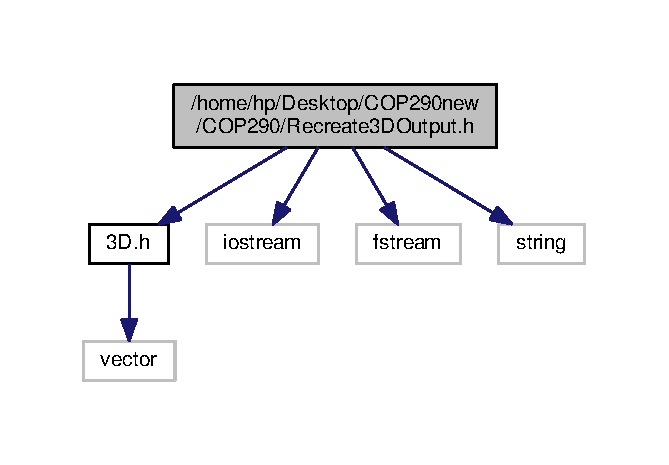
\includegraphics[width=321pt]{_recreate3_d_output_8h__incl}
\end{center}
\end{figure}
\subsection*{Functions}
\begin{DoxyCompactItemize}
\item 
void \hyperlink{_recreate3_d_output_8h_aaee408011d3a81576402bf6cc17fc631}{recreate3D} (\hyperlink{class_three_d_body}{Three\+D\+Body} threedbody)
\end{DoxyCompactItemize}


\subsection{Function Documentation}
\index{Recreate3\+D\+Output.\+h@{Recreate3\+D\+Output.\+h}!recreate3D@{recreate3D}}
\index{recreate3D@{recreate3D}!Recreate3\+D\+Output.\+h@{Recreate3\+D\+Output.\+h}}
\subsubsection[{\texorpdfstring{recreate3\+D(\+Three\+D\+Body threedbody)}{recreate3D(ThreeDBody threedbody)}}]{\setlength{\rightskip}{0pt plus 5cm}void recreate3D (
\begin{DoxyParamCaption}
\item[{{\bf Three\+D\+Body}}]{threedbody}
\end{DoxyParamCaption}
)}\hypertarget{_recreate3_d_output_8h_aaee408011d3a81576402bf6cc17fc631}{}\label{_recreate3_d_output_8h_aaee408011d3a81576402bf6cc17fc631}

\hypertarget{_reduce2_d_input_8h}{}\section{/home/hp/\+Desktop/\+C\+O\+P290new/\+C\+O\+P290/\+Reduce2\+D\+Input.h File Reference}
\label{_reduce2_d_input_8h}\index{/home/hp/\+Desktop/\+C\+O\+P290new/\+C\+O\+P290/\+Reduce2\+D\+Input.\+h@{/home/hp/\+Desktop/\+C\+O\+P290new/\+C\+O\+P290/\+Reduce2\+D\+Input.\+h}}
{\ttfamily \#include \char`\"{}2\+D.\+h\char`\"{}}\\*
{\ttfamily \#include $<$iostream$>$}\\*
{\ttfamily \#include $<$fstream$>$}\\*
{\ttfamily \#include $<$string$>$}\\*
Include dependency graph for Reduce2\+D\+Input.\+h\+:
\nopagebreak
\begin{figure}[H]
\begin{center}
\leavevmode
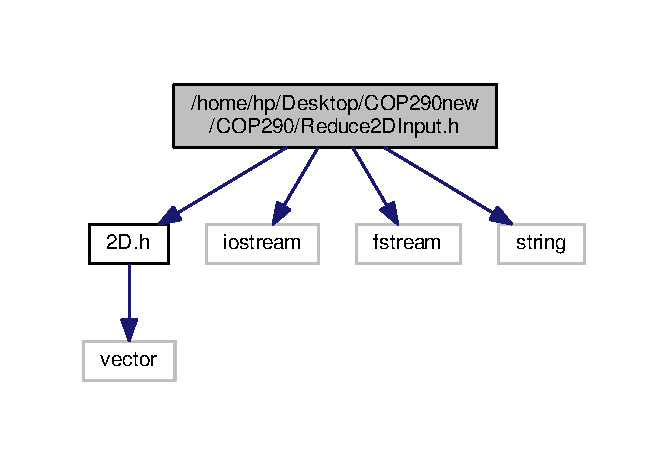
\includegraphics[width=321pt]{_reduce2_d_input_8h__incl}
\end{center}
\end{figure}
\subsection*{Functions}
\begin{DoxyCompactItemize}
\item 
\hyperlink{class_three_d_body}{Three\+D\+Body} \hyperlink{_reduce2_d_input_8h_a347b680194764814467487376063ac4c}{reduce2D} (std\+::ifstream \&Input\+File)
\end{DoxyCompactItemize}


\subsection{Function Documentation}
\index{Reduce2\+D\+Input.\+h@{Reduce2\+D\+Input.\+h}!reduce2D@{reduce2D}}
\index{reduce2D@{reduce2D}!Reduce2\+D\+Input.\+h@{Reduce2\+D\+Input.\+h}}
\subsubsection[{\texorpdfstring{reduce2\+D(std\+::ifstream \&\+Input\+File)}{reduce2D(std::ifstream &InputFile)}}]{\setlength{\rightskip}{0pt plus 5cm}{\bf Three\+D\+Body} reduce2D (
\begin{DoxyParamCaption}
\item[{std\+::ifstream \&}]{Input\+File}
\end{DoxyParamCaption}
)}\hypertarget{_reduce2_d_input_8h_a347b680194764814467487376063ac4c}{}\label{_reduce2_d_input_8h_a347b680194764814467487376063ac4c}

\hypertarget{_reduce3_d_input_8h}{}\section{/home/hp/\+Desktop/\+C\+O\+P290new/\+C\+O\+P290/\+Reduce3\+D\+Input.h File Reference}
\label{_reduce3_d_input_8h}\index{/home/hp/\+Desktop/\+C\+O\+P290new/\+C\+O\+P290/\+Reduce3\+D\+Input.\+h@{/home/hp/\+Desktop/\+C\+O\+P290new/\+C\+O\+P290/\+Reduce3\+D\+Input.\+h}}
{\ttfamily \#include \char`\"{}3\+D.\+h\char`\"{}}\\*
{\ttfamily \#include $<$iostream$>$}\\*
{\ttfamily \#include $<$fstream$>$}\\*
{\ttfamily \#include $<$string$>$}\\*
Include dependency graph for Reduce3\+D\+Input.\+h\+:\nopagebreak
\begin{figure}[H]
\begin{center}
\leavevmode
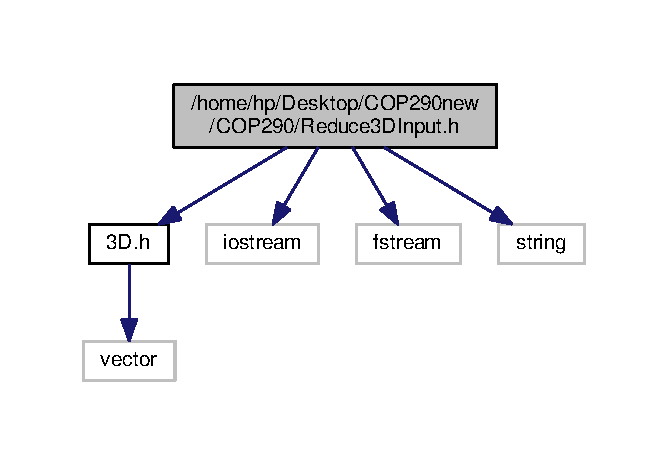
\includegraphics[width=321pt]{_reduce3_d_input_8h__incl}
\end{center}
\end{figure}
This graph shows which files directly or indirectly include this file\+:\nopagebreak
\begin{figure}[H]
\begin{center}
\leavevmode
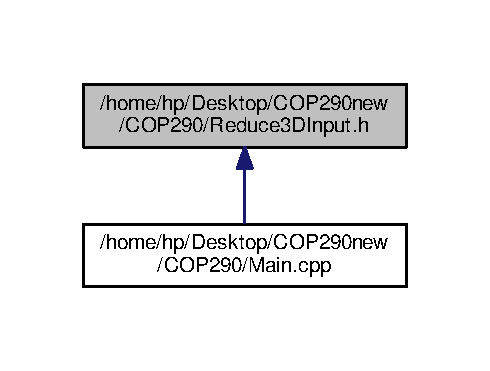
\includegraphics[width=235pt]{_reduce3_d_input_8h__dep__incl}
\end{center}
\end{figure}
\subsection*{Functions}
\begin{DoxyCompactItemize}
\item 
\hyperlink{class_three_d_body}{Three\+D\+Body} \hyperlink{_reduce3_d_input_8h_ae1d8f30412a5601f1c1e089a339bc99a}{reduce3D} (std\+::ifstream \&Input\+File)
\end{DoxyCompactItemize}


\subsection{Function Documentation}
\index{Reduce3\+D\+Input.\+h@{Reduce3\+D\+Input.\+h}!reduce3D@{reduce3D}}
\index{reduce3D@{reduce3D}!Reduce3\+D\+Input.\+h@{Reduce3\+D\+Input.\+h}}
\subsubsection[{\texorpdfstring{reduce3\+D(std\+::ifstream \&\+Input\+File)}{reduce3D(std::ifstream &InputFile)}}]{\setlength{\rightskip}{0pt plus 5cm}{\bf Three\+D\+Body} reduce3D (
\begin{DoxyParamCaption}
\item[{std\+::ifstream \&}]{Input\+File}
\end{DoxyParamCaption}
)}\hypertarget{_reduce3_d_input_8h_ae1d8f30412a5601f1c1e089a339bc99a}{}\label{_reduce3_d_input_8h_ae1d8f30412a5601f1c1e089a339bc99a}

%--- End generated contents ---

% Index
\backmatter
\newpage
\phantomsection
\clearemptydoublepage
\addcontentsline{toc}{chapter}{Index}
\printindex

\end{document}
